\documentclass[10pt,a4paper]{article}


% Nota:
% A0 bounding box: portrait 0 0 2383 3370
% A0 bounding box: landscape 0 0 3370 2383
% A4 bounding box: portrait 0 0 595 841
% A4 bounding box: landscape 0 0 841 595

% Para multiplas colunas, use o multicolumn

% \usepackage[utf8x]{inputenc}

\usepackage[brazil]{babel}
%\usepackage[latin1]{inputenc}
\usepackage[lmargin=2cm, rmargin=2cm, tmargin=2cm, bmargin=2cm]{geometry} % acerto de margens
\usepackage[scaled=.92]{helvet} % font adjusted for times size.

\usepackage{multicol}
\usepackage{array}

\usepackage{graphicx}

% \usepackage{courier} %for typewriter

% espacamento entre colunas
\setlength{\columnsep}{1cm}

\pagestyle{empty} % sem enumeracao

\newenvironment{Figure}
  {\par\medskip\noindent\minipage{\linewidth}}
  {\endminipage\par\medskip}


\begin{document}



\begin{figure}[!ht]
     \centering
     
\includegraphics[scale=1.3]{logo_emancipa.jpg}
\end{figure}

 % \large % usando tamanho grande
\begin{center}
\scalebox{2}{\scshape Simulado - Florestan Fernandes (Butant\~a)}
\end{center}

. \\

\section*{\LARGE{Instru\c{c}\~oes}}
	\begin{enumerate}
	\item  Confira se, al\'em deste caderno, voc\^e recebeu o cart\~ao destinado \`as respostas. Caso n\~ao tenha recebido, pe\c{c}a ao fiscal.
	\item Verifique se este caderno cont\'em 46 quest\~oes e uma proposta de reda\c{c}\~ao.
	\item Utilize apenas caneta esferogr\'afica azul ou preta.
	\item Cada quest\~ao proposta apresenta somente uma alternativa correta. No cart\~ao de respostas, atribuir-se-\'a pontua\c{c}\~ao zero a toda quest\~ao com mais de uma alternativa assinalada, ainda que dentre elas se encontre a correta.
	\item N\~ao \'e permitido fazer uso de instrumentos auxiliares para o c\'alculo ou portar material que sirva de consulta.
	\item O tempo dispon\'ivel para esta prova, incluindo o preenchimento do cart\~ao de respostas e a realiza\c{c}\~ao da reda\c{c}\~ao, \'e de cinco horas. Reserve os vinte minutos finais para preencher o cart\~ao de respostas.
	\item Quando terminar, entregue ao fiscal o cart\~ao de respostas, que poder\'a ser invalidado caso n\~ao esteja assinado.
	\item Em caso de d\'uvidas sobre como proceder, pe\c{c}a para falar com o fiscal. N\~ao ser\~ao esclarecidas quest\~oes relativas ao conte\'udo da prova.
	\end{enumerate}
\pagebreak


\section*{Proposta de Reda\c{c}\~ao}
	Com base na leitura dos textos motivadores seguintes e nos conhecimentos constru\'idos ao longo de sua forma\c{c}\~ao, redija um texto dissertativo-argumentativo em norma culta escrita da l\'ingua portuguesa sobre o tema \textbf{O indiv\'iduo frente \`a \'etica nacional}, apresentando proposta de a\c{c}\~ao social, que respeite os direitos humanos. Selecione, organize e relacione coerentemente argumentos e fatos para a defesa do seu ponto de vista. \\

\begin{figure}[!ht]
	\centering
     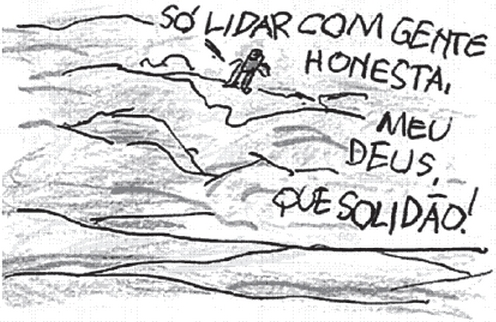
\includegraphics[scale=0.7]{redacao.jpg}
     \caption{Mill\^or Fernandes, dispon\'ivel em uol.com.br/millor/, acessado em 14 jul 2009}
     \label{redacao}
\end{figure}


Andamos demais acomodados, todo mundo reclamando em voz baixa como se fosse errado indignar-se. Sem ufanismo, que dele estou cansada, sem dizer que este \'e um pa\'is rico, de gente boa e cordata, com natureza (a que sobrou) bel\'issima e generosa - sem fantasiar nem botar \'oculos cor-de-rosa que o momento n\~ao permite, eu me pergunto o que anda acontecendo com a gente. \\
 Tenho medo disso que nos tornamos ou em que estamos nos transformando, achando bonita a ignor\^ancia eloquente, engra\c{c}ado o cinismo bem-vestido, interessante o banditismo arrojado, normal o abismo em cuja beira nos equilibramos - n\~ao malabaristas, mas palha\c{c}os. \footnote{LUFT, Ponto de Vista, Ed. 1988, 27 de dezembro de 2006 (adapta\c{c}\~ao)} \\ \\

\textbf{Qual \'e o efeito em n\'os do ``eles s\~ao todos corruptos" ?} \\
As den\'uncias que assolam nosso cotidiano podem dar lugar a uma vontade de transformar o mundo s\'o se nossa indigna\c{c}\~ao n\~ao afetar o mundo inteiro. ``Eles s\~ao TODOS corruptos" ? um pensamento que serve apenas para "confirmar" a "integridade" de quem se indigna. \\
O lugar-comum sobre a corrup\c{c}\~ao generalizada n\~ao \'e uma armadilha para os corruptos: eles continuam iguais e livres, enquanto, fechados em casa, festejamos nossa esplendorosa retid\~ao. \\
O dito lugar-comum \'e uma armadilha que amarra e imobiliza os mesmos que denunciam a imperfei\c{c}{c}\~ao do mundo inteiro. \footnote{CALLIGARIS, C. A armadilha da corrup\c{c}\~ao. Dispon\'ivel em www.folha.uol.com.br (adaptado)} \\ \\

\textbf{INSTRU\c{C}\~OES} \\
\begin{enumerate}
\item Seu texto tem de ser escrito \emph{\`a tinta}, na \emph{folha pr\'opria}.
\item Desenvolva seu texto em prosa: n\~ao redija narra\c{c}\~ao, nem poema.
\item O texto com at\'e 7 (sete) linhas escritas ser\'a considerado em branco.
\item O texto deve ter no m\'aximo \emph{30 linhas}.
\item O \emph{rascunho} da reda\c{c}\~ao dever ser feito no lugar apropriado.
\end{enumerate}
\pagebreak

\section*{Quest\~oes}


\begin{multicols}{2}

\begin{enumerate}

	%%%%%%%%%%%%%%%%%%%%%%%%%%%%%%%%%%%%%%%%%%%%%%%%%%%%%%%%%%%%%%%%%%%%%%%%%%%%%%%%%%%%
	%%%%%%%%%%%%   Matem\'atica

%*e%
	\item \textbf{Texto para esta quest\~ao e para a pr\'oxima}\\
	Em 2008, de acordo com o IBGE, 2,4\% dos brasileiros de 7 a 14 anos ainda estavam fora da escola. Embora pare\c{c}a pouco, os n\'umeros absolutos ainda assustam. ``S\~ao 680 mil crian\c{c}as sem estudar, das quais 450 mil s\~ao negras e pardas, a maioria vivendo nas Regi\~oes Norte e Nordeste", revela o soci\'ologo e presidente da Associa\c{c}\~ao dos Docentes da Universidade Federal do Amazonas (Ufam) Ant\^onio Neto, para quem esse \'e mais um item a justificar o investimento de 10\% no PIB na educa\c{c}\~ao p\'ublica. \footnote{Fonte: http://redeemancipa.org.br/2012/05/entidade-defende-10-do-pib-para-educacao/} \\ \\
O total de brasileiros com idade entre 7 e 14 anos em 2008, de acordo com o IBGE foi de aproximadamente:
		\begin{enumerate}
		\item 3000 mil
		\item 2833 mil
		\item 3 milh\~oes
		\item 283 milh\~oes
		\item 28 milh\~oes
		\end{enumerate}

%*d%
	\item Dentre as 680 mil crian\c{c}as sem estudar, a porcentagem de negras e pardas \'e de aproximadamente:

		\begin{enumerate}
		\item 7\%
		\item 37\%
		\item 53\%
		\item 66\%
		\item 82\%
		\end{enumerate}

%*b%
	\item No livro ``O homem que calculava", de Malba Tahan, o calculista Beremiz apresenta a defini\c{c}\~ao do que seria um n\'umero perfeito da seguinte maneira: ``\'e o n\'umero que apresenta a propriedade de ser igual \'e soma de seus divisores, excluindo-se, \'e claro, o pr\'oprio n\'umero. Assim, por exemplo, o n\'umero 28 apresenta 5 divisores menores que 28 (a saber, 1, 2, 4, 7 e 14). \\
	A soma desses divisores ($1+2+4+7+14$) \'e precisamente igual a 28. Logo, 28 pertence \`a  categoria dos n\'umeros perfeitos". \\
	Qual dos n\'umeros abaixo tamb\'em \'e um \textbf{n\'umero perfeito}?

		\begin{enumerate}
		\item 3
		\item 6
		\item 12
		\item 24
		\item 48
		\end{enumerate}

%*c%
	\item Joana foi, pela primeira, vez na manifesta\c{c}\~ao do 8 de mar\c{c}o (dia internacional da luta das mulheres). L\'a, ela viu um enorme cartaz com dizeres que fez com que ela sentisse muito bem. Segue, abaixo o cartaz com sua medidas:

\begin{Figure}
     \centering
     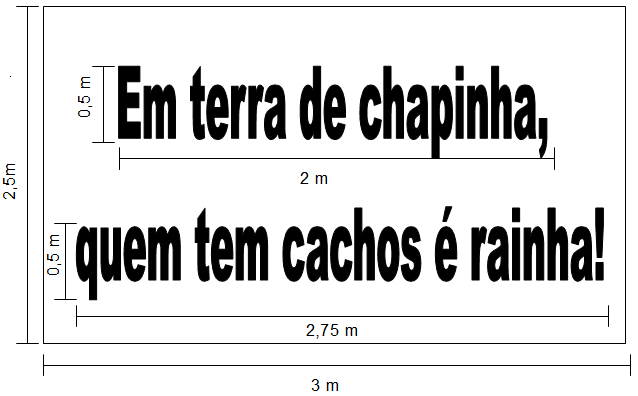
\includegraphics[width=\linewidth]{cartaz.png}
\end{Figure}

Chegando em casa, Joana quis fazer uma capa para seu caderno com os mesmos dizeres. Sabendo que a capa do caderno tem 15 cm de altura por 18 cm de comprimento, para manter a propor\c{c}\~ao do cartaz, qual deve ser a altura e o comprimento, em cm, da primeira frase (``Em terra de rainha,") e da segunda frase ("quem tem cachos \'e rainha!"), respectivamente?

		\begin{enumerate}
		\item 2 por 12 e 2 por 16,5
		\item 3 por 12 e 3 por 15,5
		\item 3 por 12 e 3 por 16,5
		\item 3 por 15 e 3 por 16,5
		\item 4 por 15 e 4 por 18,5
		\end{enumerate}
%*a%
	\item Dos 190 candidatos a prefeito nas 26 capitais brasileiras registrados no Tribunal Superior Eleitoral (TSE), apenas 28 (15\%) s\~ao mulheres. Segundo o TSE, foram feitos 198.745 registros de homens e 85.893 de mulheres para disputar vagas em todas as Câmaras Municipais do pa\'is. Para o cargo de vereador a lei imp\~oe que cada legenda tenha “o m\'inimo de 30\% e o m\'aximo de 70\% para as candidaturas de cada sexo”. \footnote{Fonte: http://www.tse.jus.br/} \\
	Se todas as candidatas e candidatos a vereadores fossem do mesmo partido a lei citada acima estaria sendo seguida?

		\begin{enumerate}
		\item sim, pois 69,8\% dos candidatos s\~ao homens e 30,2\% s\~ao mulheres.
		\item sim, pois 67,8\% dos candidatos s\~ao homens e 33,1\% s\~ao mulheres.
		\item n\~ao, pois 72,1\% dos candidatos s\~ao homens e 27,9\% s\~ao mulheres.
		\item n\~ao, pois 33,1\% dos candidatos s\~ao homens e 67,8\% s\~ao mulheres.
		\item n\~ao, pois 30,2\% dos candidatos s\~ao homens e 69,8\% s\~ao mulheres.
		\end{enumerate}

%*c%
	\item O n\'ivel sonoro $N$, medido em decib\'eis (dB), e a intensidade do som $x$, medido em watts por metro quadrado ($\frac{W}{m^2}$), est\~ao relacionados pela seguinte express\~ao:
		$$ N = 120 + 10 \cdot \log_{10} (x) $$
	Suponha que foram medidos em dois locais diferentes dois n\'iveis  sonoros $N_1$ e $N_2$, associados a duas intensidades $x_1$ e $x_2$, respectivamente.\\
	Sabendo que $N_1 - N_2 = 20dB$, qual \'e o valor do quociente $\frac{x_1}{x_2}$?
		\begin{enumerate}
		\item $10$
		\item $10^{-1}$
		\item $10^2$
		\item $10^{-2}$
		\item $10^3$
		\end{enumerate}

%*a%
	\item Marcela quer viajar, mas antes precisa contratar um seguro com cobertura de 30 mil euros. A seguradora s\'o oferece seguros com coberturas dadas em d\'olares.\\
		Considerando que 1 euro vale 2 reais e cinquenta centavos e que 1 d\'olar vale 1 real e cinquenta centavos, ela pode contratar um seguro com qual cobertura (dada em 	d\'olares)?
		\begin{enumerate}
		\item $50000$
		\item $5000$
		\item $25000$
		\item $2500$
		\item $5200$
		\end{enumerate}

%*c%
	\item A figura abaixo mostra um ret\^angulo que foi dividido em 4 quadrados. Sabendo que o comprimento do ret\^angulo \'e de 15cm, ent\~ao a largura \'e

\begin{Figure}
     \centering
     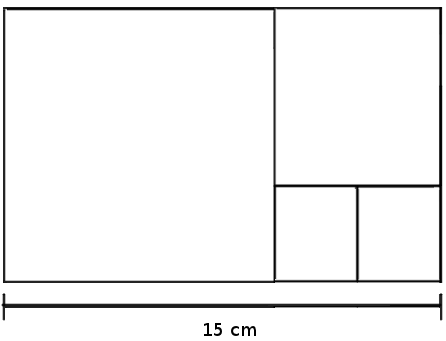
\includegraphics[width=\linewidth]{retangulo_quadrado_matematica.jpg}
\end{Figure}


		\begin{enumerate}
		\item 3cm
		\item 5cm
		\item 9cm
		\item 12cm
		\item 15cm
		\end{enumerate}



%*b%
	\item Uma pessoa de estatura mediana pretende fazer um alambrado em torno do campo de futebol de seu bairro. \\
	 No dia da medida do terreno, esqueceu de levar a trena para realizar a medi\c{c}\~ao. Para resolver o problema, a pessoa cortou uma vara de comprimento igual a sua altura. O formato do campo \'e retangular e foi constatado que ele mede 53 varas de comprimento e 30 varas de largura.\\
Uma regi\~ao R tem \'area $A_R$, dada em $m^2$, de mesma medida do campo de futebol, descrito acima. \\
A express\~ao alg\'ebrica que determina a medida da vara \'e 
		\begin{enumerate}
		\item vara = $\sqrt{\frac{A_R}{1500}}m$
		\item vara = $\sqrt{\frac{A_R}{1590}}m$
		\item vara = $\frac{1500}{A_R}m$
		\item vara = $\frac{A_R}{1500}m$
		\item vara = $\frac{A_R}{1590}m$
		\end{enumerate}



	%%%%%%%%%%%%%%%%%%%%%%%%%%%%%%%%%%%%%%%%%%%%%%%%%%%%%%%%%%%%%%%%%%%%%%%%%%%%%%%%
	%%%  Qu\'imica

%*a%
	\item Ajude a salvar o planeta, mas antes fa\c{c}a as contas:\\
	Atualmente, sistemas de purifica\c{c}\~ao de emissões poluidoras est\~ao sendo exigidos por lei em um n\'umero cada vez maior de pa\'ises. O controle das emissões de di\'oxido de enxofre gasoso, provenientes da queima de carv\~ao que cont\'em enxofre, pode ser feito pela rea\c{c}\~ao desse g\'as com uma suspens\~ao de hidr\'oxido de c\'alcio em \'agua, sendo formado um produto n\~ao poluidor do ar. \\
	A queima do enxofre e a rea\c{c}\~ao do di\'oxido de enxofre com o hidr\'oxido de c\'alcio, bem como as massas de algumas das substâncias envolvidas nessas rea\c{c}ões, podem ser assim representadas: \\
	\begin{center}
		$S$ (32 g) + $O$ (32 g) $\rightarrow SO_2$  (64 g) \\
		$SO_2$ (64 g) + $Ca(OH)_2$  (74 g) $\rightarrow$ produto n\~ao poluidor
	\end{center}
   onde $S$ \'e enxofre, $O$ \'e \'oxigênio, $SO_2$ \'e di\'oxido de enxofre e $Ca(OH)_2$ \'e hidr\'oxido de c\'alcio.\\
	Dessa forma, para absorver todo o di\'oxido de enxofre produzido pela queima de uma tonelada de carv\~ao (contendo 1\% de enxofre), \'e suficiente a utiliza\c{c}\~ao de uma massa de hidr\'oxido de c\'alcio de, aproximadamente, 
	\begin{enumerate}
	\item 23 kg.
	\item 43 kg.
	\item 64 kg.
	\item 74 kg.
	\item 138 kg.
	\end{enumerate}

%*e%
	\item Considere os seguintes acontecimentos ocorridos no Brasil. Ao final, conclua sobre pol\'iticas corretas de gerenciamento de produtos qu\'imicos e radioativos.\\

a) Goi\'as, 1987 - Um equipamento contendo c\'esio radioativo, utilizado em medicina nuclear (isto \'e, antes do acidentes muitas pessoas foram ajudadas), foi encontrado em um dep\'osito de sucatas e aberto por pessoa que desconhecia o seu conte\'udo. \\
Resultado: mortes e consequências ambientais sentidas at\'e hoje. \\

b) Distrito Federal, 1999 - Cilindros contendo cloro, g\'as bactericida utilizado em tratamento de \'agua, encontrados em um dep\'osito de sucatas, foram abertos por pessoa que desconhecia o seu conte\'udo. \\
Resultado: mortes, intoxica\c{c}ões e consequências ambientais sentidas por v\'arias horas.\\
Para evitar que novos acontecimentos dessa natureza venham a ocorrer, foram feitas as seguintes
propostas para a atua\c{c}\~ao do Estado:\\

I. Proibir o uso de materiais radioativos e gases t\'oxicos. \\
II. Controlar rigorosamente a compra, uso e destino de materiais radioativos e de recipientes contendo gases t\'oxicos. \\
III. Instruir usu\'arios sobre a utiliza\c{c}\~ao e descarte destes materiais.\\
IV. Realizar campanhas de esclarecimentos \`a popula\c{c}\~ao sobre os riscos da radia\c{c}\~ao e da toxicidade de determinadas substâncias. \\
V. Proibir produtos qu\'imicos.\\

	Dessas respostas, s\~ao adequadas apenas:
		\begin{enumerate}
		\item I, III e V.
		\item I, II e V.
		\item II e III
		\item I, III e IV.
		\item II, III e IV.
		\end{enumerate}



%*d%
	\item Quando definem mol\'eculas, os livros geralmente apresentam conceitos como: ``a menor parte da substância capaz de guardar suas propriedades". \\
	A partir de defini\c{c}ões desse tipo, a ideia transmitida ao estudante \'e a de que o constituinte isolado (mol\'eculas) cont\'em os atributos do todo.\\
	\'E como dizer que uma mol\'ecula de \'agua possui densidade, press\~ao de vapor, tens\~ao superficial, ponto de fus\~ao, ponto de ebuli\c{c}\~ao, etc. Tais propriedades pertencem ao conjunto, isto \'e, manifestam-se nas rela\c{c}ões que as mol\'eculas mantêm entre si. \footnote{Adaptado de OLIVEIRA, R. J. O Mito da Substância. Qu\'imica Nova na Escola, n. o 1, 1995.}

	
	O texto anterior evidencia a chamada vis\~ao substancialista que ainda se encontra presente no ensino da Qu\'imica.\\
	Abaixo est\~ao relacionadas algumas afirmativas pertinentes ao assunto. 

I. O ouro \'e dourado, pois seus \'atomos s\~ao dourados. Da mesma forma, os \'atomos de prata s\~ao prateados.\\
II. Uma substância ``macia" n\~ao pode ser feita de mol\'eculas ``r\'igidas".\\
III. Uma substância pura possui pontos de ebuli\c{c}\~ao e fus\~ao constantes, em virtude das intera\c{c}ões entre suas mol\'eculas.\\
IV. A expans\~ao dos objetos com a temperatura ocorre porque os \'atomos se expandem.\\

Dessas afirmativas, est\~ao apoiadas na vis\~ao substancialista criticada pelo autor apenas:
	\begin{enumerate}
	\item I e II.
	\item III e IV.
	\item I, II e III.
	\item I, II e IV.
	\item II, III e IV. 
	\end{enumerate}


%*b%
	\item  \begin{center} A Mat\'eria est\'a cheia de Vazio !!!! \end{center}
		``Em n\'ivel subatômico, substancias aparentemente s\'olidas como a madeira, o a\c{c}o ou as pedras contem um enorme espa\c{c}o vazio. Neste artigo, o F\'isico e escritor cientifico inglês Paul Davies, nos conduz a uma fascinante viagem pelo interior da mat\'eria e de seus mist\'erios ainda n\~ao perfeitamente decifrados pela ciência..."\footnote{Superinteressante – SETEMBRO de 1993}\\
	Com rela\c{c}\~ao a afirma\c{c}\~ao contida na introdu\c{c}\~ao do artigo acima, que \'e verdadeira, assinale a explica\c{c}\~ao correta:
		\begin{enumerate}
		\item \'Atomos e mol\'eculas s\~ao pequenos e \'infimos quando comparados \`a estrutura macrosc\'opica de substâncias iônicas ou covalentes.
		\item No interior do \'atomo, o que mais existe \'e espa\c{c}o vazio, pois o n\'ucleo atômico \'e \'infimo quando comparado ao \'atomo. 
		\item \'Atomos e mol\'eculas s\~ao muito separados entre si, provocando grandes espa\c{c}os vazios na mat\'eria.
		\item Nêutrons s\~ao respons\'aveis pelos espa\c{c}os vazios.
		\item Os nêutrons do n\'ucleo s\~ao muito pequenos quando comparados aos pr\'otons.
		\end{enumerate}



%*b%
	\item \begin{quote}``A idade da pedra chegou ao fim, n\~ao porque faltassem pedras; a era do petr\'oleo chegar\'a igualmente ao fim, mas n\~ao por falta de petr\'oleo" \footnote{Xeque Yamani, Ex-ministro do Petr\'oleo da Ar\'abia Saudita. O Estado de S. Paulo, 20/08/2001.} \end{quote}
	Considerando as caracter\'isticas que envolvem a utiliza\c{c}\~ao das mat\'erias-primas citadas no texto em diferentes contextos hist\'orico-geogr\'aficos, \'e correto afirmar que, de acordo com o autor, a exemplo do que aconteceu na Idade da Pedra, o fim da era do Petr\'oleo estaria relacionado
		\begin{enumerate}
		\item \`a redu\c{c}\~ao e esgotamento das reservas de petr\'oleo. 
		\item ao desenvolvimento tecnol\'ogico e \`a utiliza\c{c}\~ao de novas fontes de energia. 
		\item ao desenvolvimento dos transportes e conseqüente aumento do consumo de energia. 
		\item ao excesso de produ\c{c}\~ao e conseqüente desvaloriza\c{c}\~ao do barril de petr\'oleo. 
		\item \`a diminui\c{c}\~ao das a\c{c}ões humanas sobre o meio ambiente. 
		\end{enumerate}

%*d%
	\item O \'acido sulf\'idrico, como \'e popularmente tratado e que \'e sua solu\c{c}\~ao aquosa, ocorre naturalmente no petr\'oleo cru, g\'as natural, gases vulcânicos, e mananciais de \'aguas termais (pr\'oximas a vulc\~oes). Tamb\'em pode ocorrer como resultado da degrada\c{c}\~ao bacteriana de mat\'eria orgânica em condi\c{c}\~oes anaer\'obicas. Se gera a partir de alguns amino\'acidos ou pela redu\c{c}\~ao de sulfatos presentes em microrganismos sulfatoredutores, produto de dejetos animais e humanos. \\
	As bact\'erias que se encontram na boca e no trato gastrointestinal, produzem \'acido sulf\'idrico, ao degradar materiais que cont\'em prote\'inas vegetais e animais. O \'acido sulf\'idrico pode ser produzido por atividades industriais, tais como processamento aliment\'icio, coquerias, f\'abricas de papel, curtumes e refinarias de petr\'oleo.\\
	O \'acido sulf\'idrico ($H_2S$) \'e um g\'as inflam\'avel, incolor, com odor caracter\'istico a ovos podres (desagrad\'avel). Com refer\^encia \`a mol\'ecula $H_2S$, forne\c{c}a a distribui\c{c}\~ao eletr\^onica fundamental de cada elemento ($H=1$; $S=16$)

		\begin{enumerate}
		\item $ _1H - 1p^1 / _{16}S - 1S^2 \  2S^2 \ 2p^6 \ 3S^2 \ 3p^4$
		\item $ _1H - 1s^1 / _{16}S - 1S^2 \  2S^4 \ 2p^6 \ 3S^2 \ 3p^4$
		\item $ _1H - 1s^1 / _{16}S - 1S^2 \  2S^2 \ 2p^4 \ 3S^6 \ 3p^4$
		\item $ _1H - 1s^1 / _{16}S - 1S^2 \  2S^2 \ 2p^6 \ 3S^2 \ 3p^4$
		\item Nenhuma das anteriores.
		\end{enumerate}

%*c%
	\item Os fulerenos s\~ao uma forma \textbf{ alotr\'opica} do \textbf{ Carbono}, a terceira mais est\'avel ap\'os o diamante e o grafite. Tornaram-se populares entre os qu\'imicos, tanto pela sua beleza estrutural quanto pela sua versatilidade para a s\'intese de novos compostos qu\'imicos. A estrutura dos fulerenos \'e formada pela liga\c{c}\~ao das bordas de uma folha de \emph{grafeno}. Desse modo, os carbonos continuam unidos por fortes liga\c{c}\~oes $sp^2$, como no grafeno, entretanto a curvatura trigonal das liga\c{c}\~oes leva a forma\c{c}\~ao de uma estrutura pseudo $sp^3$. Esta apresenta a forma de uma bola de futebol formada por \textbf{ hex\'agonos} (20) interligados por \textbf{ pent\'agonos} (12), sendo estes \'ultimos respons\'aveis pela curvatura da mol\'ecula e, consequentemente, por sua forma tridimensional. Por isso, tal estrutura tamb\'em \'e conhecida como ``futeboleno".

\begin{Figure}
     \centering
     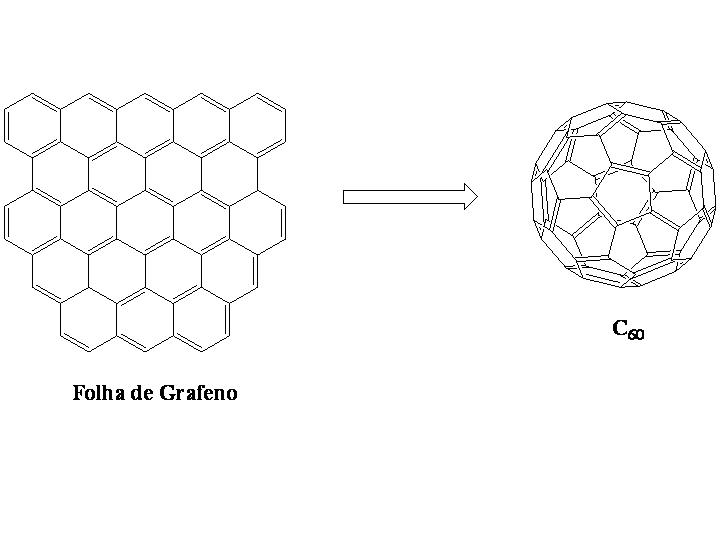
\includegraphics[width=\linewidth]{futeboleno_quimica.jpg}
\end{Figure}

	O representante mais conhecido e est\'avel da fam\'ilia dos fulerenos \'e o $C_{60}$: 60 \'atomos de carbono dispostos na forma de um \emph{icosaedro}. Em rela\c{c}\~ao aos tipos de hibridiza\c{c}\~oes de orbitais que os \'atomos de carbono presentes nesta mol\'ecula, podemos afirmar que:


		\begin{enumerate}
		\item a hibridiza\c{c}\~ao do tipo $sp^2$ resulta em 2 orbitais $sp^2$ e 2 orbitais p
		\item a hibridiza\c{c}\~ao do tipo $sp^3$ resulta em 2 orbitais $sp^3$ e 2 orbitais p
		\item a hibridiza\c{c}\~ao do tipo $sp^2$ resulta em 3 orbitais $sp^2$ e 1 orbital p
		\item a hibridiza\c{c}\~ao do tipo $sp^3$ resulta em 1 orbitais $sp^3$ e 3 orbitais p
		\item a hibridiza\c{c}\~ao do tipo $sp^3$ resulta em 2 orbitais $sp^3$ e 2 orbitais p
		\end{enumerate}
%*e%
	\item O acetileno, conhecido pela nomenclatura IUPAC por etino, \'e um hidrocarboneto da classe dos alcinos. Devido a sua queima extremamente exot\'ermica, \'e usado em larga escala na solda autog\^enica, no corte de metais por ma\c{c}arico, na fabrica\c{c}\~ao de objetos de vidro e em diversos processos que requeiram altas temperaturas. No ma\c{c}arico oxiacetil\^enico obt\^em-se temperaturas de 2500 a 3000°C. \\
	Dentre suas aplica\c{c}\~oes na ind\'ustria qu\'imica como mat\'eria-prima, encontra-se a s\'intese de centenas de compostos, dentre os quais os mais destacados s\~ao o etileno, o etanol, diversos compostos organoclorados, especialmente solventes como o clorof\'ormio e o \'acido ac\'etico. \'E utilizado tamb\'em na produ\c{c}\~ao de borracha sint\'etica e pol\'imeros. Com base na estrutura molecular deste composto \'e incorreto afirmar que:

		\begin{enumerate}
		\item as liga\c{c}\~oes ente os \'atomos de carbono s\~ao 3 sigma ($\sigma$)
		\item as liga\c{c}\~oes ente os \'atomos de carbono s\~ao 3 pi ($\pi$)
		\item as liga\c{c}\~oes ente os \'atomos de carbono s\~ao 2 sigma ($\sigma$)
		\item as liga\c{c}\~oes ente os \'atomos de carbono s\~ao 3 pi ($\pi$)
		\item as liga\c{c}\~oes ente os \'atomos de carbono s\~ao 2 pi ($\pi$)
		\end{enumerate}

%*b%
	\item O benzeno e o cicloexano (olhar as figuras abaixo) s\~ao solventes utilizados em laborat\'orio. Comparando-se as caracter\'isticas desses dois compostos, \'e incorreto afirmar que:

\begin{Figure}
     \centering
     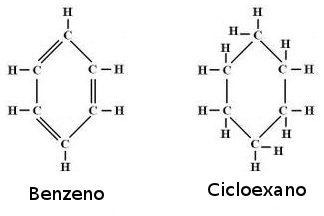
\includegraphics[width=\linewidth]{benzeno_cicloexano_quimica.jpg}
\end{Figure}

		\begin{enumerate}
		\item ambos s\~ao constitu\'idos por mol\'eculas de seis \'atomos de carbono
		\item  ambos s\~ao hidrocarbonetos arom\'aticos
		\item ambos s\~ao l\'iquidos \`a temperatura de 25 ºC
		\item a mol\'ecula de benzeno tem liga\c{c}\~oes pi ($\pi$) e a do cicloexano s\'o tem liga\c{c}\~oes sigma ($\sigma$)
		\item no benzeno, os \'atomos de C apresentam hibridiza\c{c}\~ao $sp^2$ e, no cicloexano, $sp^3$
		\end{enumerate}

%*e%
	\item Uma das subst\^ancias l\'iquidas cristalinas mais eficientes, empregadas na produ\c{c}\~ao de Visores de Cristal L\'iquido (LCD), \'e o composto 

\begin{Figure}
     \centering
     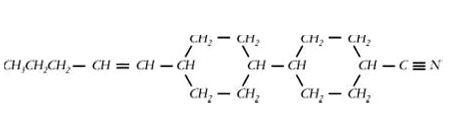
\includegraphics[width=\linewidth]{composto_quimica.jpg}
\end{Figure}

	Em rela\c{c}\~ao a esse composto, \'e incorreto afirmar: 

		\begin{enumerate}
		\item a f\'ormula molecular \'e $C_{18}H_{29}N$ 
		\item o n\'umero de \'atomos de carbono (C) prim\'ario (ligado somente a outro C), secund\'ario (ligado a outros dois C) e terci\'ario (ligado a tr\^es C) \'e, respectivamente, 2, 12 e 4.
		\item o n\'umero de \'atomos de carbono com hibridiza\c{c}\~ao $sp^3$, $sp^2$ e $sp$ \'e, respectivamente, 15, 2 e 1.
		\item o n\'umero de liga\c{c}\~oes pi ($\pi$) \'e igual a 3 
		\item apenas os \'atomos de carbono terci\'arios possuem geometria tetra\'edrica 
		\end{enumerate}



	%%%%%%%%%%%%%%%%%%%%%%%%%%%%%%%%%%%%%%%%%%%%%%%%%%%%%%%%%%%%%%%%%%%%%%%%%%%%%%%%%%%%
	%%%%%%%%%%%%   F\'isica

%*b%	
	\item O metano \'e um g\'as nocivo \`a atmosfera terrestre por agravar o efeito estufa. Com base no gr\'afico abaixo, assinale a alternativa correta.

\begin{Figure}
     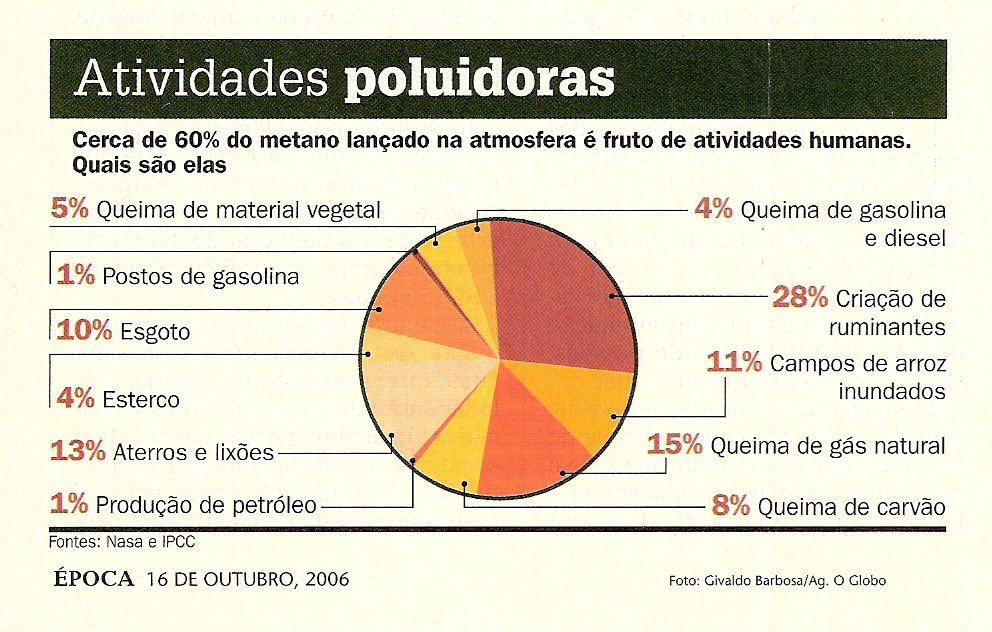
\includegraphics[scale=0.235]{ozonio.jpg}
\end{Figure}

		\begin{enumerate}
		\item A emiss\~ao de metano devido \`a cria\c{c}\~ao de ruminantes \'e maior que a emiss\~ao de metano devido a queima de g\'as natural e carv\~ao juntas
		\item O esterco emite mais metano que a queima de apenas \'oleo diesel
		\item A produ\c{c}\~ao de petr\'oleo est\'a entre as atividades que mais liberam metano na atmosfera
		\item 40\% do metano lan\c{c}ado na atmosfera \'e fruto de atividades humanas
		\item A cria\c{c}\~ao de ruminantes \'e a atividade que menos libera metano na atmosfera
		\end{enumerate}

%*d%
	\item Apesar de ser um pa\'is com enorme oferta de recursos naturais, o Brasil enfrenta problemas de energia el\'etrica. Com base no gr\'afico abaixo, \'e correto afirmar que:

\begin{Figure}
     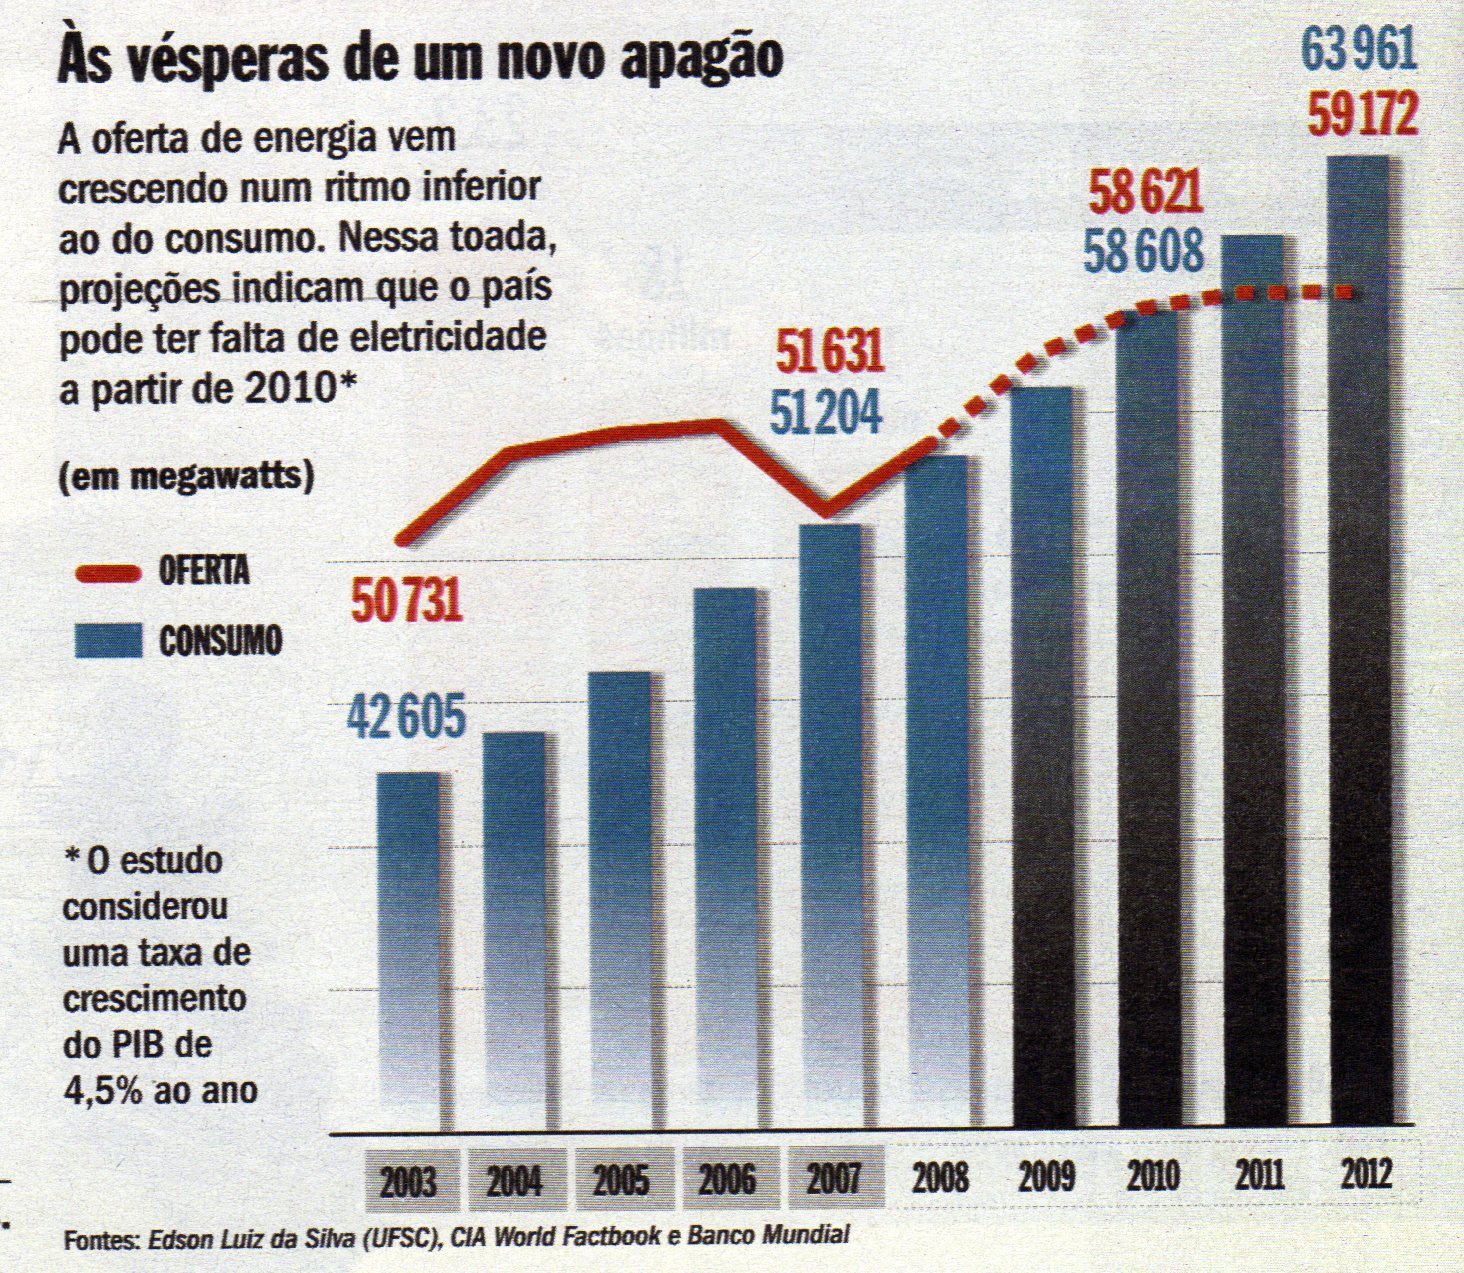
\includegraphics[width=\linewidth]{apagao.jpg}
\end{Figure}


		\begin{enumerate}
		\item A oferta de energia el\'etrica era maior em 2007 que em 2006.
		\item A oferta de energia sempre esteve abaixo do consumo.
		\item Em 2005, o consumo de energia era de 50731 megawatts.
		\item O consumo de energia sempre aumentou.
		\item Segundo as previs\~oes, o pa\'is poder\'a ter um apag\~ao a partir de 2012.
		\end{enumerate}

%*c%
	\item Um autom\'ovel e um \^onibus trafegam em uma estrada plana, mantendo velocidades constantes em torno de 100 km/h e 75 km/h, respectivamente. Os dois ve\'iculos passam lado a lado em um posto de ped\'agio. Quarenta minutos ($\frac{2}{3}$ de hora) depois, nessa mesma estrada, o motorista do \^onibus v\^e o autom\'ovel ultrapass\'a-lo. Ele sup\~oe, ent\~ao, que o autom\'ovel deve ter realizado, nesse per\'iodo, uma parada com dura\c{c}\~ao aproximada de
		\begin{enumerate}
		\item 4 minutos
		\item 7 minutos
		\item 10 minutos
		\item 15 minutos
		\item 25 minutos
		\end{enumerate}

%*d%
	\item Um passageiro, viajando de metr\^o, fez o registro de tempo entre duas esta\c{c}\~oes e obteve os valores indicados na tabela. \\


	\begin{Figure}  % tabela
	\begin{tabular}{|c|c|c|} % aqui temos 3 colunas centralizadas
	\hline
	& Chegada  & Partida \tabularnewline
	
	\hline
	 Vila Maria & 0:00 min & 1:00 min \tabularnewline

	\hline
	  Felicidade & 5:00 min & 6:00 min \tabularnewline
	\hline
	\end{tabular}
	\end{Figure}

	Supondo que a velocidade m\'edia entre duas esta\c{c}\~oes consecutivas seja sempre amesma e que o trem pare o mesmo tempo em qualquer esta\c{c}\~ao da linha, de 15 km de extens\~ao, \'e poss\'ivel estimar que um trem, desde a partida da Esta\c{c}\~ao Bosque at\'e a chegada \`a Esta\c{c}\~ao Terminal, leva aproximadamente
	

\begin{Figure}
     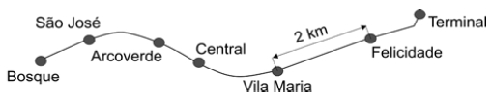
\includegraphics[width=\linewidth]{cidades_fisica.jpg}
\end{Figure}

		\begin{enumerate}
		\item 20 minutos
		\item 25 minutos
		\item 30 minutos
		\item 35 minutos
		\item 40 minutos
		\end{enumerate}


%*a%
	\item Todo carro possui uma caixa de fus\'iveis. Os fus\'iveis s\~ao elementos utilizados para prote\c{c}\~ao de circuitos el\'etricos. Os fus\'iveis s\~ao constitu\'idos de material de baixo ponto de fus\~ao, como o estanho, por exemplo, e se fundem quando percorridos por uma corrente el\'etrica igual ou maior do que aquela que s\~ao capazes de suportar, ou seja ele n\~ao permite que uma corrente el\'etrica maior do que a que ele \'e capaz de suportar passe para o circuito.  O quadro a seguir mostra uma s\'erie de fus\'iveis e os valores de corrente por ele suportados.

	\begin{Figure}  % tabela
	\begin{tabular}{|c|c|} % aqui temos 2 colunas centralizadas
	\hline
	 Fus\'ivel  & Corrente el\'etrica (A) \tabularnewline
	\hline
	 Azul & 1,5 \tabularnewline
	\hline
	 Amarelo & 2,5  \tabularnewline
	\hline
	  Laranja & 5,0	   \tabularnewline
	\hline
	 Preto & 7,5 \tabularnewline
	\hline
	 Vermelho & 10,0 \tabularnewline
	\hline
	\end{tabular}
	\end{Figure}

	Para proteger o resistor de 12 ohm indicado na figura abaixo, qual o menor valor de fus\'ivel que pode ser escolhido.

\begin{Figure}
     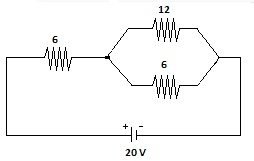
\includegraphics[width=\linewidth]{circuito_fisica.jpg}
\end{Figure}



		\begin{enumerate}
		\item Azul
		\item Amarelo
		\item Laranja
		\item  Preto
		\item Vermelho
		\end{enumerate}


%*a%
	\item  Em circutos el\'etricos muitas vezes n\~ao est\'a dispon\'ivel a resist\^encia el\'etrica com o valor de resist\^encia exatamente como se deseja. Por exemplo, pode ser que se queira uma resist\^encia de 2 Ohm mas s\'o h\'a dispon\'ivel resist\^encias de 1 ohm, e portanto \'e feita uma liga\c{c}\~ao em s\'erie com duas resist\^encias de 1 Ohm. Associa\c{c}\~ao de resist\^encias em s\'erie ou em paralelo s\~ao muito utilizadas no dia-a-dia. No circuito abaixo qual o valor da corrente i2 e quais tipos de associa\c{c}\~ao de resist\^encias est\~ao presentes no circuito.

\begin{Figure}
     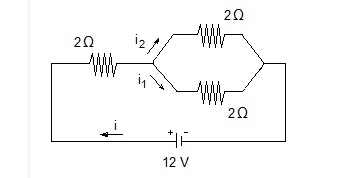
\includegraphics[width=\linewidth]{circuito_2_fisica.jpg}
\end{Figure}

		\begin{enumerate}
		\item 2 amp\'ere; s\'erie e paralelo
		\item 2 amp\'ere; apenas s\'erie
		\item 1,5 amp\'ere; apenas paralelo
		\item 3 amp\'ere; apenas s\'erie
		\item 3 amp\'ere; s\'erie e paralelo
		\end{enumerate}
%*b%
	\item Mariazinha sempre ajuda a sua m\~ae a ir fazer compras no supermecardo. Um dia a m\~ae de Mariazinha pediu que ela fosse no a\c{c}ougue comprar 2kg de carne, e para isso ela lhe deu R\$10,00. Ao caminho do supermercado ela teve que passar por uma sorveteria e decidiu comprar um picol\'e que custava R\$1,00. Chegando ao a\c{c}ougue ela descobriu que o quilo de carne custava R\$ 6,00. Supondo que ela compre todo o dinheiro que lhe restou em carne, quantos quilos de carne ela ir\'a conseguir levar para casa?
		\begin{enumerate}
		\item 1 kg
		\item 1 kg e 500 g
		\item 2 kg
		\item 2 kg e 500 g
		\item 3 kg
		\end{enumerate}

%*e%
	\item Bianca comprou 3 camisetas e pagou R\$ 120,00. Quanto ela pagaria se comprasse 5 camisetas de mesmo tipo e pre\c{c}o?
		\begin{enumerate}
		\item R\$ 120,00
		\item R\$ 140,00
		\item R\$ 160,00
		\item R\$ 180,00
		\item R\$ 200,00
		\end{enumerate}


	%%%%%%%%%%%%%%%%%%%%%%%%%%%%%%%%%%%%%%%%%%%%%%%%%%%%%%%%%%%%%%%%%%%%%%%%%%%%%%%
	%%%%%%%%%%%%%%%   Hist\'oria

%*a%
	\item  Em meio \`as turbul\^encias vividas na primeira metade dos anos 1960, tinha-se a impress\~ao de que 
as tend\^encias de esquerda estavam se fortalecendo na \'area cultural. O Centro Popular de Cultura (CPC) da Uni\~ao Nacional dos Estudantes (UNE) encenava pe\c{c}as de teatro que faziam agita\c{c}\~ao e propaganda em favor da luta pelas reformas de base e satirizavam  o ``imperialismo" e seus ``aliados internos".\footnote{KONDER, L. Hist\'oria das Ideias Socialistas no Brasil. S\~ao Paulo: Express\~ao Popular, 2003.}\\
	No in\'icio da d\'ecada de 1960, enquanto v\'arios setores da esquerda brasileira consideravam 
que o CPC da UNE era uma importante forma de conscientiza\c{c}\~ao das classes trabalhadoras, 
os setores conservadores e de direita (pol\'iticos vinculados \`a Uni\~ao Democr\'atica Nacional - UDN -, 
Igreja Cat\'olica, grandes empres\'arios, etc) entendiam que esta organiza\c{c}\~ao:
		\begin{enumerate}
		\item constitu\'ia mais uma amea\c{c}a para a democracia brasileira, ao difundir a ideologia comunista.
		\item contribu\'ia com a valoriza\c{c}\~ao da genu\'ina cultura nacional, ao encenar pe\c{c}as de cunho popular.
		\item realizava uma tarefa que deveria ser exclusiva do Estado, ao pretender educar o povo por meio da cultura.
		\item prestava um servi\c{c}o importante \`a sociedade brasileira, ao incentivar a participa\c{c}\~ao pol\'itica dos 
mais pobres.
		\item diminu\'ia a for\c{c}a dos oper\'arios urbanos, ao substituir os sindicatos como institui\c{c}\~ao de press\~ao pol\'itica sobre o governo.
		\end{enumerate}

%*d%
	\item \'E dif\'icil encontrar um texto sobre a Proclama\c{c}\~ao  da rep\'ublica no Brasil que n\~ao cite a afirma\c{c}\~ao de Aristides Lobo, no Di\'ario Popular de S\~ao Paulo, de que ``o povo assistiu \`aquilo bestializado". Essa vers\~ao foi relida pelos enaltecedores da Revolu\c{c}\~ao de 1930, que n\~ao descuidaram da forma rep\'ublicana, mas real\c{c}aram a exclus\~ao social, o militarismo e o estrangeirismo da f\'ormula implantada em 1889. Isto porque o Brasil brasileiro teria nascido em 1930. \footnote{MELLO, M. T. C. A rep\'ublica consentida: cultura democr\'atica e cient\'ifica no final do imp\'erio, Rio de Janeiro: FGV, 2007 (adaptado).} \\
	O texto defende que a consolida\c{c}\~ao de uma determinada mem\'oria sobre a Proclama\c{c}\~ao da Rep\'ublica no Brasil teve, na Revolu\c{c}\~ao de 1930, um de seus momentos mais importantes. Os defensores da Revolu\c{c}\~ao de 1930 procuraram construir uma vis\~ao negativa para os eventos de 1889, porque esta era uma maneira de
		\begin{enumerate}
		\item valorizar as propostas pol\'iticas democr\'aticas e liberais vitoriosas.
		\item resgatar simbolicamente as figuras politicas ligadas \`a Monarquia.
		\item criticar a pol\'itica educacional adotada durante a Rep\'ublica Velha.
		\item legitimar a ordem pol\'itica inaugurada com a chegada desse grupo ao poder.
		\item destacar a ampla participa\c{c}\~ao popular obtida no processo da Proclama\c{c}\~ao.
		\end{enumerate}

%*e%
	\item Completamente analfabeto, ou quase, sem assist\^encia m\'edica, n\~ao lendo jornais, nem revistas,
 nas quais se limita a ver figuras, o trabalhador rural n\~ao ser em casos espor\'adicos, tem o patr\~ao na conta 
de benfeitor. No plano pol\'itico, ele luta com o ``coronel" e pelo ``coronel". A\'i est\~ao os votos de cabresto, que resultam, em grande parte, da nossa organiza\c{c}\~ao econ\^omica rural. \footnote{LEAL, V. N. Coronelismo, enxada e voto. S\~ao Paulo: Alfa-Ômega, 1978 (adaptado).} \\
	O coronelismo, fen\^omeno pol\'itico da Primeira Rep\'ublica (1889-1930), tinha como uma de suas principais caracter\'isticas o controle do voto, o que limitava, portanto, o exerc\'icio da cidadania. Nesse per\'iodo, esta pr\'atica estava vinculada a uma estrutura social

		\begin{enumerate}
		\item igualit\'aria, com um n\'ivel satisfat\'orio de distribui\c{c}\~ao da renda.
		\item estagnada, com uma relativa harmonia entre as classes.   
		\item tradicional, com a manuten\c{c}\~ao da escravid\~ao nos engenhos como forma produtiva t\'ipica.
		\item ditatorial, perturbada por um constante clima de opress\~ao mantido pelo ex\'ercito e pol\'icia.
		\item agr\'aria, marcada pela concentra\c{c}\~ao da terra e do poder pol\'itico local e regional.
		\end{enumerate}

%*c%
	\item No Conc\'ilio de Clermont (em 27 de novembro de 1095), o papa Urbano II lan\c{c}ou um apelo aos crist\~aos, com a seguinte prega\c{c}\~ao:
		\begin{quote}
		Deixai os que outrora estavam acostumados a se baterem, impiedosamente contra os fi\'eis, em guerras particulares, lutarem contra os infi\'eis. (...) Deixai os que at\'e aqui foram ladr\~oes tornarem-se soldados. Deixai aqueles que outrora se bateram contra seus irm\~aos e parentes lutarem agora contra os b\'arbaros como devem. (...) Tomai o caminho do Santo Sepulcro, arrebatai aquela terra \`a ra\c{c}a perversa e submetei-a a v\'os mesmos
		\end{quote} 
	Neste discurso, o papa Urbano II conclamou os crist\~aos organizarem expedi\c{c}\~oes de resist\^encia aos considerados ``infi\'eis" que controlavam ``lugares santos". Genericamente, quem eram os ``infi\'eis", como foram chamadas estas expedi\c{c}\~oes e, al\'em dos motivos religiosos, quais foram as inspira\c{c}\~oes econ\^omicas? 

		\begin{enumerate}
	       \item Os ``infi\'eis", genericamente, eram os mul\c{c}umanos. As expedi\c{c}\~oes eram denominadas Cruzadas, e que possu\'iam como inspira\c{c}\~ao econ\^omica, por exemplo, a acumula\c{c}\~ao de moedas de ouro e prata do oriente.
		\item Os ``infi\'eis", genericamente, eram os africanos. As expedi\c{c}\~oes eram denominadas Cruzadas, e que possu\'iam como inspira\c{c}\~ao econ\^omica a conquista de escravos de guerra.
		\item Os ``infi\'eis", genericamente, eram os mul\c{c}umanos. Cruzadas \'e a denomina\c{c}\~ao utilizada para se referir a esta s\'erie de expedi\c{c}\~oes realizadas pelos crist\~aos com o prop\'osito econ\^omico de, por exemplo,  reabrir e dominar rotas comerciais.
		\item Genericamente, os ``infi\'eis" eram os mu\c{c}ulmanos e as expedi\c{c}\~oes eram chamadas de peregrina\c{c}\~oes. Possu\'iam motiva\c{c}\~oes econ\^omicas diversas, muitas delas estavam intimamente ligadas \`a acumula\c{c}\~ao de itens religiosos que possu\'iam grande capital simb\'olico.
		\item Genericamente, os ``infi\'eis" eram os mu\c{c}ulmanos e as expedi\c{c}\~oes eram chamadas de cruzadas. Possu\'iam motiva\c{c}\~oes econ\^omicas diversas, dentre elas a realiza\c{c}\~ao de trocas comerciais em todo o oceano atlântico
		\end{enumerate}

%*d%
	\item Leia o texto a seguir sobre a cultura medieval.
		\begin{quote}
		A ci\^encia perdeu a vitalidade e a velha uni\~ao com a filosofia se dissolveu (...) A filosofia contraiu nova alian\c{c}a, dessa vez com a teologia, durante s\'eculos a vida intelectual se processaria sobre a orienta\c{c}\~ao da igreja (...) \'E cab\'ivel indagar da Hist\'oria se h\'a alguma raz\~ao v\'alida para supor que o g\^enio humano chamejou com menos brilho quando os homens , por boas raz\~oes (...) da \'epoca, transferiram o pensamento especulativo da ci\^encia-filosofia para a teologia-filosofia. Presumivelmente, os homens do (...) princ\'ipio da Idade M\'edia nasceram com a mesma capacidade de pensar, inquirir e evoluir intelectualmente que os homens de qualquer outra \'epoca. A quest\~ao, ent\~ao, n\~ao \'e se tinham capacidade, mas se podiam ou desejavam us\'a-la e como a usavam. \footnote{William Carrol Bark. Origens da Idade M\'edia.
 Trad. 3 ed. Rio de Janeiro: Zahar, 1974. P. 102-3.}
		\end{quote}
	Em suas considera\c{c}\~oes a respeito da cultura medieval, o autor do texto questiona a ideia que se generalizou de que a Idade M\'edia foi uma longa ``Idade das Trevas". Essa concep\c{c}\~ao se deveu, em parte, ao fato de:

		\begin{enumerate}
		\item A cultura medieval ter se limitado a reproduzir a cultura dos cl\'assicos e n\~ao ter criado novas formas de express\~ao. 
		\item A filosofia e a teologia terem sido desvalorizados na Idade M\'edia porque dificultavam o avan\c{c}o da ci\^encia.  
		\item Os medievos terem exercitado pouco suas capacidades intelectuais, dedicando-se mais a guerra e a religi\~ao. 
		\item A express\~ao Idade M\'edia ter sido usada pelos renascentistas, que retomavam valores culturais do per\'iodo cl\'assico Greco-romano.
		\item A cultura produzida na Idade M\'edia ter sido uma s\'intese das culturas cl\'assicas, germânicas e \'arabes. 
		\end{enumerate}

%*d%
	\item ``A experi\^encia dos nossos tempos mostra que os pr\'incipes que tiveram pouco respeito pela boa f\'e puderam com ast\'ucia confundir os esp\'iritos e chegaram a superar os que basearam sua conduta na lealdade (...) Um governante prudente n\~ao dever\'a agir com boa f\'e quando, para faz\^e-lo, precise trabalhar contra seus interesses, e quando os motivos que o levaram a contrair uma obriga\c{c}\~ao deixarem de existir. Este preceito n\~ao seria justo se todos os homens fossem bons; mas como eles s\~ao maus e n\~ao mant\^em palavra, n\~ao se est\'a obrigado a agir com boa f\'e." \footnote{MAQUIAVEL, O Pr\'incipe. Bras\'ilia: editora da UNB, 1979. P. 76} \\

	Considerando o ambiente cultural do Renascimento e o trecho da obra de Maquiavel citado acima, identifique a alternativa correta.

		\begin{enumerate}
		\item  O pensamento renascentista n\~ao apresentava car\'ater cr\'itico, raz\~ao pela qual n\~ao podemos classificar \emph{O Pr\'incipe}, de Maquiavel, como uma obra cr\'itica.
		\item Como uma aut\^entica produ\c{c}\~ao renascentista, a an\'alise de Maquiavel sobre a pol\'itica desconsiderava as motiva\c{c}\~oes humanistas, destacando as explica\c{c}\~oes de cunho moral e \'etnico. 
		\item N\~ao podemos classificar Maquiavel como um autor renascentista porque toda a sua obra era de car\'ater puramente ficcional. 
		\item Podemos identificar no texto de Maquiavel duas das principais caracter\'isticas do Renascimento: o racionalismo e o individualismo.
		\item De acordo com \emph{O Pr\'incipe}, Maquiavel difundia o princ\'ipio de que os governantes deveriam agir com lealdade. 
		\end{enumerate}

%*a%
	\item A extra\c{c}\~ao do ouro aparentemente simples atraiu milhares de pessoas para a Am\'erica Portuguesa cuja popula\c{c}\~ao estimada passou de 300.000 habitantes em 1690 para 2.500.000 em 1780. Metade deste aumento demogr\'afico ocorreu na regi\~ao mineradora. Considerando essas informa\c{c}\~oes pode-se afirmar que:

		\begin{enumerate}
		\item O denominado ``ciclo do ouro" possibilitou uma esp\'ecie de atra\c{c}\~ao centr\'ipeta para o mercado interno desenvolvido pela minera\c{c}\~ao e assim contribuiu como fator de integra\c{c}\~ao regional na Am\'erica Portuguesa.  
		\item A popula\c{c}\~ao atra\'ida para a minera\c{c}\~ao tamb\'em desenvolveu intensa atividade agr\'aria de subsist\^encia propiciando reconhecida auto-sufici\^encia que inibiu qualquer tipo de polariza\c{c}\~ao.  
		\item O Regimento dos Superintendentes / Guardas-Mores e Oficiais Deputados para as Minas que em 1702 instituiu a Intend\^encia das Minas mantinha rigorosa disciplina militar e constante vigilância na Estrada Real impedindo o ingresso de emboabas e mascates nas regi\~oes de ouro e diamante
		\item O denominado ``ciclo do ouro" ocasionou uma esp\'ecie de atra\c{c}\~ao centr\'ifuga pois as riquezas aur\'iferas de Goi\'as e da Bahia contribu\'iram para financiar simultaneamente o denominado renascimento agr\'icola no Nordeste do Brasil no final do s\'eculo XVII. 
		\item A integra\c{c}\~ao regional da Am\'erica Portuguesa consolidou-se durante a Uni\~ao Ib\'erica (1580-1640) quando foi removida a linha de Tordesilhas possibilitando a converg\^encia das regi\~oes de pecu\'aria para o grande entreposto comercial que consagrou a regi\~ao de Minas Gerais.
		\end{enumerate}

%*b%
	\item ``O primeiro grupo social utilizado pelos portugueses como escravo foi o das comunidades ind\'igenas encontradas no Brasil. A l\'ogica era simples: os \'indios estavam localizados junto ao litoral, e o custo inicial era pequeno, se comparado ao trabalhador origin\'ario de Portugal. (...) \\
No entanto, rapidamente ocorreu um decl\'inio no emprego do trabalhador ind\'igena." \footnote{Rubim Santos Le\~ao de Aquino et al, Sociedade brasileira: uma hist\'oria atrav\'es dos movimentos sociais} \\
	O decl\'inio a que o texto se refere e o avan\c{c}o da explora\c{c}\~ao do trabalhador escravo africano podem ser explicados: 

		\begin{enumerate}
		\item pelo preju\'izo que a escraviza\c{c}\~ao ind\'igena gerava para os senhores de engenho que tinham a obriga\c{c}\~ao da catequese; pela impossibilidade de a Coroa portuguesa cobrar tributos nos neg\'ocios envolvendo os nativos da col\^onia; pela presen\c{c}a de uma pequena comunidade ind\'igena nas regi\~oes produtoras de a\c{c}\'ucar.
		\item pela forte oposi\c{c}\~ao dos jesu\'itas \`a escraviza\c{c}\~ao indiscriminada dos \'indios; pelo lucro da Coroa portuguesa e dos traficantes com o com\'ercio de africanos; pela necessidade de fornecimento regular de m\~ao de obra para a atividade a\c{c}ucareira, em franca expans\~ao na passagem do s\'eculo XVI ao XVII.   
		\item pela imposi\c{c}\~ao de escravos do norte da \'Africa, por parte dos grandes traficantes holandeses; pela determina\c{c}\~ao da Igreja cat\'olica em proibir a escraviza\c{c}\~ao ind\'igena em todo Imp\'erio colonial portugu\^es; pelo custo menor do escravo de algumas regi\~oes da \'Africa, como Angola e Guin\'e.
		\item pelos preceitos das Ordena\c{c}\~oes Filipinas, que indicavam o caminho da catequese e n\~ao o do trabalho para os nativos americanos; pelo desconhecimento, por parte dos \'indios brasileiros, de uma economia de mercado; pelos acordos entre o colonizador portugu\^es e parte das lideran\c{c}as ind\'igenas.
		\item pela extrema fragilidade f\'isica dos povos ind\'igenas encontrados nas terras portuguesas na Am\'erica; pelos preceitos religiosos da Contra-Reforma, que n\~ao aceitavam a escraviza\c{c}\~ao de povos primitivos; pela impossibilidade de encontrar e capturar \'indios no interior do espa\c{c}o colonial. 
		\end{enumerate}

%*b%
	\item Em rela\c{c}\~ao ao per\'iodo da ocupa\c{c}\~ao holandesa no Nordeste brasileiro, afirma-se: \\
		I. A invas\~ao deveu-se aos interesses dos comerciantes holandeses pelo a\c{c}\'ucar produzido na regi\~ao, interesses esses que foram prejudicados devido \`a Uni\~ao Ib\'erica (1580-1640). \\
		II. Foi, tamb\'em, uma consequ\^encia dos conflitos econ\^omicos e pol\'iticos que envolviam as rela\c{c}\~oes entre os chamados Pa\'ises Baixos e o Imp\'erio espanhol. \\
		III. As medidas econ\^omicas de Nassau garantiam os lucros da Companhia das \'Indias Ocidentais e os lucros dos senhores de engenho, j\'a que aumentaram a produ\c{c}\~ao do a\c{c}\'ucar. \\
		IV. A pol\'itica adotada por Nassau para assentar os holandeses na Bahia acabou por deflagrar sua derrota e o fim da ocupa\c{c}\~ao holandesa, gra\c{c}as \`a resist\^encia dos \'indios e portugueses expulsos das terras que ocupavam. \\
	S\~ao verdadeiras as proposi\c{c}\~oes: 
		\begin{enumerate}
		\item I e II.
		\item I, II e III.
		\item II, III e IV.
		\item I, III e IV.
		\item II e IV.
		\end{enumerate}





	%%%%%%%%%%%%%%%%%%%%%%%%%%%%%%%%%%%%%%%%%%%%%%%%%%%%%%%%%%%%%%%%%%%%%%%%%%%%%%%%%%%%%%%%5
	%%%%%%%%%%%%  Portugu\^es

%*c%
	\item Aumento do efeito estufa amea\c{c}a plantas, diz estudo. O aumento de di\'oxido de carbono na atmosfera, resultante do uso de combust\'iveis f\'osseis e das queimadas, pode ter \emph{consequ\^encias calamitosas} para o clima mundial, \emph{mas} tamb\'em pode afetar diretamente o crescimento das plantas. \emph{Cientistas} da Universidade de Basel, na Su\'i\c{c}a, mostraram que, \emph{embora} o di\'oxido de carbono seja essencial para o crescimento dos vegetais, quantidades excessivas desse \emph{g\'as} prejudicam a sa\'ude das plantas e t\^em efeitos incalcul\'aveis na agricultura de v\'arios pa\'ises. \footnote{O Estado de S\~ao Paulo, 20 set. 1992, p.32. } \\
	O texto acima possui elementos coesivos que promovem sua manuten\c{c}\~ao tem\'atica. A partir dessa perspectiva, conclui-se que 

		\begin{enumerate}
		\item a palavra ``mas" (em it\'alico) contradiz a afirma\c{c}\~ao inicial do texto: linhas 1 e 2.
		\item a palavra ``embora" (em  it\'alico) introduz uma explica\c{c}\~ao que n\~ao encontra complemento no restante do texto.
		\item as express\~oes: ``consequ\^encias calamitosas", na linha 2, e ``efeitos incalcul\'aveis", na linha 6, refor\c{c}am a ideia que perpassa o texto sobre o perigo do efeito estufa.
		\item o uso da palavra ``cientistas" (em it\'alico) \'e desnecess\'ario para dar credibilidade ao texto, uma vez que se fala em ``estudo" no t\'itulo do texto.
		\item a palavra ``g\'as" (em it\'alico), refere-se a ``combust\'iveis f\'osseis" e "queimadas", nas linhas primeiras linhas do texto, refor\c{c}ando a ideia de cat\'astrofe.
		\end{enumerate}

%*b%
	\item A sociedade atual testemunha a influ\^encia determinante das tecnologias digitais na vida do homem moderno, sobretudo daquelas relacionadas com o computador e a internet. Entretanto, parcelas significativas da popula\c{c}\~ao n\~ao t\^em acesso a tais tecnologias. Essa limita\c{c}\~ao tem pelo menos dois motivos: a impossibilidade financeira de custear os aparelhos e os provedores de acesso, e a impossibilidade de saber utilizar o equipamento e usufruir das novas tecnologias. A essa problem\'atica, d\'a-se o nome de exclus\~ao digital. \\
No contexto das pol\'iticas de inclus\~ao digital, as escolas, nos usos pedag\'ogicos das tecnologias de informa\c{c}\~ao, devem estar voltadas principalmente para 
		\begin{enumerate}
		\item  proporcionar aulas que capacitem os estudantes a montar e desmontar computadores, para garantir a compreens\~ao sobre o que s\~ao as tecnologias digitais.
		\item  explorar a facilidade de ler e escrever textos e receber coment\'arios na internet para desenvolver a interatividade e a an\'alise cr\'itica, promovendo a constru\c{c}\~ao do conhecimento.
		\item estudar o uso de programas de processamento para imagens e v\'ideos de alta complexidade para capacitar profissionais em tecnologia digital.
		\item estudar o uso de programas de processamento para imagens e v\'ideos de alta complexidade para capacitar profissionais em tecnologia digital.
		\item  estimular as habilidades psicomotoras relacionadas ao uso f\'isico do computador, como mouse, teclado, monitor etc.
		\end{enumerate}

%*e%
	\item Os filhos de Ana eram bons, uma coisa verdadeira e sumarenta. Cresciam, tomavam banho, exigiam para si, malcriados, instantes cada vez mais completos. Acozinha era enfim espa\c{c}osa, o fog\~ao engui\c{c}ado dava estouros. O calor era forte no apartamento que estavam aos poucos pagando. Mas o vento batendo nas cortinas que ela mesma cortara lembrava-lhe que se quisesse podia parar e enxugar a testa, olhando o calmo horizonte. Como um lavrador. Ela plantara as sementes que tinha na m\~ao, n\~ao outras, mas essas apenas. \footnote{LISPECTOR, C. La\c{c}os de fam\'ilia. Rio de Janeiro: Rocco, 1998.} \\
	A autora emprega por duas vezes o conectivo mas no fragmento apresentado. Observando aspectos da organiza\c{c}\~ao, estrutura\c{c}\~ao e funcionalidade dos elementos que articulam o texto, o conectivo mas expressa o mesmo conte\'udo nas duas situa\c{c}\~oes em que aparece no texto, o conectivo mas:
		
		\begin{enumerate}
		\item expressa o mesmo conte\'udo nas duas situa\c{c}\~oes em que aparece no texto.
		\item quebra a fluidez do texto e prejudica a compreens\~ao, se usado no in\'icio da frase.
		\item ocupa posi\c{c}\~ao fixa, sendo inadequado seu uso na abertura da frase.
		\item cont\'em uma ideia de sequ\^encia temporal que direciona a conclus\~ao do leitor.
		\item assume fun\c{c}\~oes discursivas distintas nos dois contextos de uso.
		\end{enumerate}


%*e%
	\item \textbf{Texto 1}\\
		Alguns leitores poder\~ao achar que a linguagem desta Gram\'atica se afasta do padr\~ao estrito usual neste tipo de livro. Assim, o autor escreve tenho que reformular, e n\~ao tenho de reformular; pode-se colocar dois constituintes, e n\~ao podem-se colocar dois constituintes; e assim por diante. Isso foi feito de caso pensado, com a preocupa\c{c}\~ao de aproximar a linguagem da gram\'atica do padr\~ao atual brasileiro presente nos textos t\'ecnicos e jornal\'isticos de nossa \'epoca.
	\footnote{ALMEIDA, N. M. Gram\'atica met\'odica da l\'ingua portuguesa. Pref\'acio. S\~ao Paulo: Saraiva, 1999 (adaptado).} \\
	\textbf{ Texto 2} \\
	Alguns leitores poder\~ao achar que a linguagem desta Gram\'atica se afasta do padr\~ao estrito usual neste tipo de livro. Assim, o autor escreve tenho que reformular, e n\~ao tenho de reformular; pode-se colocar dois constituintes, e n\~ao podem-se colocar dois constituintes; e assim por diante. Isso foi feito de caso pensado, com a preocupa\c{c}\~ao de aproximar a linguagem da gram\'atica do padr\~ao atual brasileiro presente nos textos t\'ecnicos e jornal\'isticos de nossa \'epoca.
	\footnote{REIS, N. Nota do editor. PERINI, M. A. Gram\'atica descritiva do portugu\^es. S\~ao Paulo: \'Atica, 1996.}\\
	Confrontando-se as opini\~oes defendidas nos dois textos, conclui-se que
		\begin{enumerate}
		\item ambos os textos tratam da quest\~ao do uso da l\'ingua com o objetivo de criticar a linguagem do brasileiro.
		\item os dois textos defendem a ideia de que o estudo da gram\'atica deve ter o objetivo de ensinar as regras prescritivas da l\'ingua.
		\item a quest\~ao do portugu\^es falado no Brasil \'e abordada nos dois textos, que procuram justificar como \'e correto e aceit\'avel o uso coloquial do idioma.
		\item o primeiro texto enaltece o padr\~ao estrito da l\'ingua, ao passo que o segundo defende que a linguagem jornal\'istica deve criar suas pr\'oprias regras gramaticais.
		\item o primeiro texto prega a rigidez gramatical no uso da l\'ingua, enquanto o segundo defende uma adequa\c{c}\~ao da l\'ingua escrita ao padr\~ao atual brasileiro.
		\end{enumerate}

%*e%
	\item \textbf{A partida}\\
		Acordei pela madrugada. A princ\'ipio com tranquilidade, e logo com obstina\c{c}\~ao, quis novamente dormir. In\'util, o sono esgotara-se. Com precau\c{c}\~ao, acendi um f\'osforo: passava das tr\^es. Restava-me, portanto, menos de duas horas, pois o trem chegaria \`as cinco. Veio-me ent\~ao o desejo de n\~ao passar mais nem uma hora naquela casa. Partir, sem dizer nada, deixar quanto antes minhas cadeias de disciplina e de amor.\\
	Com receio de fazer barulho, dirigi-me \`a cozinha, lavei o rosto, os dentes, penteei-me e, voltando ao meu quarto, vesti-me. Calcei os sapatos, sentei-me um instante \`a beira da cama. Minha av\'o continuava dormindo. Deveria fugir ou falar com ela? Ora, algumas palavras... Que me custava acord\'a-la, dizer-lhe adeus? \footnote{LINS, O. A partida. Melhores contos. Sele\c{c}\~ao e pref\'acio de Sandra Nitrini. S\~ao Paulo: Global, 2003.} \\

		
	No texto, o personagem narrador, na imin\^encia da partida, descreve a sua hesita\c{c}\~ao em separar-se da av\'o. Esse sentimento contradit\'orio fica claramente expresso no trecho:

		\begin{enumerate}
		\item ``A princ\'ipio com tranquilidade, e logo com obstina\c{c}\~ao, quis novamente dormir"
		\item ``Restava-me, portanto, menos de duas horas, pois o trem chegaria \`as cinco"
		\item ``Calcei os sapatos, sentei-me um instante \`a beira da cama"
		\item ``Partir, sem dizer nada, deixar quanto antes minhas cadeias de disciplina e amor"
		\item ``Deveria fugir ou falar com ela? Ora, algumas palavras..."
		\end{enumerate}

%*e%
	\item \textbf{ Testes} \\
		Dia desses resolvi fazer um teste proposto por um site da internet. O nome do teste era tentador: ``O que Freud diria de voc\^e". Uau. Respondi a todas as perguntas e o resultado foi o seguinte: ``Os acontecimentos da sua infância a marcaram at\'e os doze anos, depois disso voc\^e buscou conhecimento intelectual para seu amadurecimento". Perfeito! Foi exatamente o que aconteceu comigo. Fiquei radiante: eu havia realizado uma consulta paranormal com o pai da psican\'alise, e ele acertou na mosca. Estava com tempo sobrando, e curiosidade \'e algo que n\~ao me falta, ent\~ao resolvi voltar ao teste e responder tudo diferente do que havia respondido antes. Marquei umas alternativas esdr\'uxulas, que nada tinham a ver com minha personalidade. E fui conferir o resultado, que dizia o seguinte: ``Os acontecimentos da sua infância a marcaram at\'e os 12 anos, depois disso voc\^e buscou conhecimento intelectual para seu amadurecimento".
\footnote{MEDEIROS, M. Doidas e santas. Porto Alegre, 2008 (adaptado).} \\

	Quanto \`as influ\^enicas  que a internet pode exercer sobre os usu\'arios, a autora expressa uma rea\c{c}\~ao ir\^onica no trecho:

		\begin{enumerate}
		\item ``Marquei umas alternativas esdr\'uxulas, que nada tinham a ver"
		\item ``Os acontecimentos da sua infância a marcaram at\'e os doze anos"
		\item ``Dia desses resolvi fazer um teste proposto por um site da internet"
		\item ``Respondi a todas as perguntas e o resultado foi o seguinte"
	       \item ``Fiquei radiante: eu havia realizado uma consulta paranormal com o pai da psican\'alise"
		\end{enumerate}

%*d%
	\item Oximoro, ou paradoxismo, \'e uma figura de ret\'orica em que se combinam palavras de sentido oposto que parecem excluir-se mutuamente, mas que, no contexto, refor\c{c}am a express\~ao. \footnote{Dicion\'ario Eletr\^onico Houaiss da L\'ingua Portuguesa.} \\
		Considerando a defini\c{c}\~ao apresentada, o fragmento po\'etico da obra Cantares, de Hilda Hilst, publicada em 2004, em que pode ser encontrada a referida figura de ret\'orica \'e:
		\begin{enumerate}
		\item ``Dos dois contemplo \\
			rigor e fixidez.\\
			Passado e sentimento\\
			me contemplam" (p. 91).
		\item ``De sol e lua\\
			De fogo e vento \\
			Te enla\c{c}o" (p. 101).
		\item ``Areia, vou sorvendo \\
			A \'agua do teu rio" (p. 93)
		\item ``Ritualiza a matan\c{c}a \\
			de quem s\'o te deu vida. \\
			E me deixa viver \\
			nessa que morre" (p. 62)
		\item ``O bisturi e o verso. \\
			Dois instrumentos\\
			entre as minhas m\~aos" (p. 95).
		\end{enumerate}


%*a%
	\item .
		 \begin{center} \emph{Cap\'itulo III} \end{center}
		Um criado trouxe o caf\'e. Rubi\~ao pegou na x\'icara e, enquanto lhe deitava a\c{c}\'ucar, ia disfar\c{c}adamente mirando a bandeja, que era de prata lavrada. Prata, ouro, eram os metais que amava de cora\c{c}\~ao; n\~ao gostava de bronze, mas o amigo Palha disse-lhe que era mat\'eria de pre\c{c}o, e assim se explica este par de figuras que aqui est\'a na sala: um Mefist\'ofeles e um Fausto. Tivesse, por\'em, de escolher, escolheria a bandeja, - primor de argentaria, execu\c{c}\~ao fina e acabada. O criado esperava teso e s\'erio. Era espanhol; e n\~ao foi sem resist\^encia que Rubi\~ao o aceitou das m\~aos de Cristiano; por mais que lhe dissesse que estava acostumado aos seus crioulos de Minas, e n\~ao queria l\'inguas estrangeiras em casa, o amigo Palha insistiu, demonstrando-lhe a necessidade de ter criados brancos. Rubi\~ao cedeu com pena. O seu bom pajem, que ele queria p\^or na sala, como um peda\c{c}o da prov\'incia, nem o p\^ode deixar na cozinha, onde reinava um franc\^es, Jean; foi degradado a outros servi\c{c}os. \footnote{ASSIS, M. Quincas Borba. In: Obra completa. V.1. Rio de Janeiro: Nova Aguilar, 1993
(fragmento).}\\

		Quincas Borba situa-se entre as obras-primas do autor e da literatura brasileira. No fragmento apresentado, a peculiaridade do texto que garante a universaliza\c{c}\~ao de sua abordagem reside

		\begin{enumerate}
		\item no conflito entre o passado pobre e o presente rico, que simboliza o triunfo da apar\^encia sobre a ess\^encia.
		\item no sentimento de nostalgia do passado devido \`a substitui\c{c}\~ao da m\~ao de obra escrava pela dos imigrantes.
		\item na refer\^encia a Fausto e Mefist\'oteles, que representam o desejo de eterniza\c{c}\~ao de Rubi\~ao.
		\item na admira\c{c}\~ao dos metais por parte de Rubi\~ao, que metaforicamente representam a durabilidade dos bens produzidos pelo trabalho.
		\item na resist\^encia de Rubi\~ao aos criados estrangeiros, que reproduz o sentimento de xenofobia.
		\end{enumerate}


%*b%
	\item
	\begin{quote}
	 	\begin{center} \textbf{Os poemas} \end{center}
		Os poemas s\~ao p\'assaros que chegam\\
		n\~ao se sabe de onde e pousam\\
		no livro que l\^es.\\
		Quando fechas o livro, eles al\c{c}am voo\\
		como de um al\c{c}ap\~ao.\\
		Eles n\~ao t\^em pouso\\
		nem porto\\
		alimentam-se um instante em cada par de m\~aos\\
		e partem.\\
		E olhas, ent\~ao, essas tuas m\~aos vazias,\\
		no maravilhado espanto de saberes\\
		que o alimento deles j\'a estava em ti... \footnote{M\'ARIO QUINTANA 
Poesia completa. Rio de Janeiro: Nova Aguilar, 2005}
	\end{quote}
	$$ -------------------  $$
	\begin{quote}
	E olhas, ent\~ao, essas tuas m\~aos vazias, \\
no maravilhado espanto de saberes \\
que o alimento deles j\'a estava em ti... (v. 10-12) \\
	\end{quote}
	De acordo com esses versos, um dos efeitos da compreens\~ao da leitura \'e: 
		\begin{enumerate}
		\item alimentar o leitor com novas perspectivas e op\c{c}\~oes
		\item revelar ao leitor suas pr\'oprias sensa\c{c}\~oes e pensamentos
		\item transformar o leitor em uma pessoa melhor e mais consciente
		\item deixar o leitor maravilhado com a beleza e o encantamento do poema
		\item revelar ao leitor que os p\'assaros foram embora
		\end{enumerate}


%*b%
	\item \begin{quote}
		\textbf{ RECEITA DE MULHER}\\
		\\
		As muito feias que me perdoem\\
		Mas beleza \'e fundamental. \'E preciso\\
		Que haja qualquer coisa de flor em tudo isso\\
		Qualquer coisa de dan\c{c}a, qualquer coisa de haute couture\\
		Em tudo isso (ou ent\~ao\\
		Que a mulher se socialize elegantemente em azul, como na Rep\'ublica Popular Chinesa).\\
		N\~ao h\'a meio-termo poss\'ivel. \'E preciso\\
		Que tudo isso seja belo. \'E preciso que s\'ubito\\
		Tenha-se a impress\~ao de ver uma gar\c{c}a apenas pousada e que um rosto\\
		Adquira de vez em quando essa cor s\'o encontr\'avel no terceiro minuto da aurora. \footnote{Vin\'icius de Moraes, ``haute couture" (alta costura).}\\
		\end{quote}
	No conhecido poema ``Receita de mulher", de que  se reproduziu aqui um excerto, o tratamento dado ao tema da beleza feminina manifesta a 

		\begin{enumerate}
		\item oscila\c{c}\~ao do poeta entre a ang\'ustia do pecador (tendo em vista sua educa\c{c}\~ao jesu\'itica) e o impudor do libertino. 
		\item conjuga\c{c}\~ao, na sensibilidade do poeta, de interesse sexual e encantamento est\'etico, expresso de modo provocador e bem-humorado.
		\item idealiza\c{c}\~ao da mulher a que chega o poeta quando, na velhice, arrefeceu-lhe o desejo sexual. 
		\item cr\'itica ao car\'ater fr\'ivolo que, por associar-se ao consumo, o amor assume na contemporaneidade. 
		\item s\'intese, pela via do erotismo, das tend\^encias europeizantes e nacionalistas do autor.
		\end{enumerate}

%*c%
	\item Instru\c{c}\~ao: As duas pr\'oximas quest\~oes tomam por base fragmentos de um livro do b\'ulgaro Tzvetan Todorov (1939-), linguista e te\'orico da literatura. \\
	\begin{center} \textbf{ A literatura em perigo} \end{center} 
	A an\'alise das obras feita na escola n\~ao deveria mais ter por objetivo ilustrar os conceitos rec\'em-introduzidos por este ou aquele linguista, este ou aquele te\'orico da literatura, quando, ent\~ao, os textos s\~ao apresentados como uma aplica\c{c}\~ao da l\'ingua e do discurso; sua tarefa deveria ser a de nos fazer ter acesso ao sentido dessas obras — pois postulamos que esse sentido, por sua vez, nos conduz a um conhecimento do humano, o qual importa a todos. Como j\'a o disse, essa ideia n\~ao \'e estranha a uma boa parte do pr\'oprio mundo do ensino; mas \'e necess\'ario passar das ideias \`a a\c{c}\~ao. Num relat\'orio estabelecido pela Associa\c{c}\~ao dos Professores de Letras, podemos ler: “O estudo de Letras implica o estudo do homem, sua rela\c{c}\~ao consigo mesmo e com o mundo, e sua rela\c{c}\~ao com os outros.” Mais exatamente, o estudo da obra remete a c\'irculos conc\^entricos cada vez mais amplos: o dos outros escritos do mesmo autor, o da literatura nacional, o da literatura mundial; mas seu contexto final, o mais importante de todos, nos \'e efetivamente dado pela pr\'opria exist\^encia humana. Todas as grandes obras, qualquer que seja sua origem, demandam uma reflex\~ao dessa dimens\~ao.\\
  O que devemos fazer para desdobrar o sentido de uma obra e revelar o pensamento do artista? Todos os “m\'etodos” s\~ao bons, desde que continuem a ser meios, em vez de se tornarem fins em si mesmos. (...)(...)(...) \\
	Sendo o objeto da literatura a pr\'opria condi\c{c}\~ao humana, aquele que a l\^e e a compreende se tornar\'a n\~ao um especialista em an\'alise liter\'aria, mas um conhecedor do ser humano. Que melhor introdu\c{c}\~ao \`a compreens\~ao das paix\~oes e dos comportamentos humanos do que uma imers\~ao na obra dos grandes escritores que se dedicam a essa tarefa h\'a mil\^enios? E, de imediato: que melhor prepara\c{c}\~ao pode haver para todas as profiss\~oes baseadas nas rela\c{c}\~oes humanas? Se entendermos assim a literatura e orientarmos dessa maneira o seu ensino, que ajuda mais preciosa poderia encontrar o futuro estudante de direito ou de ci\^encias pol\'iticas, o futuro assistente social ou psicoterapeuta, o historiador ou o soci\'ologo? Ter como professores Shakespeare e S\'ofocles, Dostoievski e Proust n\~ao \'e tirar proveito de um ensino excepcional? E n\~ao se v\^e que mesmo um futuro m\'edico, para exercer o seu of\'icio, teria mais a aprender com esses mesmos professores do que com os manuais preparat\'orios para concurso que hoje determinam o seu destino? Assim, os estudos liter\'arios encontrariam o seu lugar no cora\c{c}\~ao das humanidades, ao lado da hist\'oria dos eventos e das ideias, todas essas disciplinas fazendo progredir o pensamento e se alimentando tanto de obras quanto de doutrinas, tanto de a\c{c}\~oes pol\'iticas quanto de muta\c{c}\~oes sociais, tanto da vida dos povos quanto da de seus indiv\'iduos. Se aceitarmos essa finalidade para o ensino liter\'ario, o qual n\~ao serviria mais unicamente \`a reprodu\c{c}\~ao dos professores de Letras, podemos facilmente chegar a um acordo sobre o esp\'irito que o deve conduzir: \'e necess\'ario incluir as obras no grande di\'alogo entre os homens, iniciado desde a noite dostempos e do qual cada um de n\'os, por mais \'infimo que seja, ainda participa. ``\'E nessa comunica\c{c}\~ao inesgot\'avel, vitoriosa do espa\c{c}o e do tempo, que se afirma o alcance universal da literatura", escrevia Paul B\'enichou. A n\'os, adultos, nos cabe transmitir \`as novas gera\c{c}\~oes essa heran\c{c}a fr\'agil, essas palavras que ajudam a viver melhor. \footnote{Tzvetan Todorov. A literatura em perigo. 2 ed.Trad. Caio Meira. Rio de Janeiro: DIFEL, 2009, p. 89-94.} \\
	\\
	Observe as seguintes opini\~oes referentes ao ensino de literatura.\\
	I. O estudo de obras liter\'arias na escola tem como objetivo fundamental ensinar os fundamentos da Lingu\'istica.\\
	II. A an\'alise das obras feita na escola deve levar o estudante a ter acesso ao sentido dessas obras.\\
	III. O objetivo do ensino da literatura na escola n\~ao \'e formar te\'oricos da literatura.\\
	IV. De nada adianta a leitura das obras liter\'arias sem a pr\'evia fundamenta\c{c}\~ao das teorias liter\'arias.\\
	Das quatro opini\~oes, as que se enquadram na argumenta\c{c}\~ao manifestada por Todorov em seu texto est\~ao contidas apenas em:
		\begin{enumerate}
		\item I e II
		\item I e III
		\item II e III
		\item I, II e  III
		\item II, III e  IV
		\end{enumerate}

%*d%
	\item Ter como professores Shakespeare e S\'ofocles, Dostoievski e Proust n\~ao \'e tirar proveito de um ensino excepcional? \\
	Esta quest\~ao levantada por Todorov, no contexto do terceiro par\'agrafo, significa:
		\begin{enumerate}
		\item O conhecimento enciclop\'edico desses autores, manifestado em suas obras, equivale a um verdadeiro curso universit\'ario.
		\item Por se tratar de autores de nacionalidades e \'epocas diferentes, a leitura de suas obras traz conhecimentos importantes sobre seus respectivos pa\'ises.
		\item Esses autores escreveram com a inten\c{c}\~ao fundamental de passar ensinamentos para seus contemporâneos e a posteridade.
		\item A leitura das obras desses autores, que focalizam admiravelmente o homem e o humano, seria de excepcional utilidade para os estudantes de rela\c{c}\~oes humanas.
		\item A leitura desses autores n\~ao acrescenta nada de excepcional ao ensino.
		\end{enumerate}

%*b%
	\item As dimens\~oes continentais do Brasil s\~ao objeto de reflex\~oes expressas em diferentes  linguagens. Esse tema aparece no seguinte poema: \\
	\begin{quote}
	(....)\\
Que importa que uns falem mole descansado\\
Que os cariocas arranhem os erres na garganta\\
Que os capixabas e paroaras escancarem as vogais?\\
Que tem se o quinhentos r\'eis meridional\\
Vira cinco tost\~oes do Rio pro Norte?\\
Junto formamos este assombro de mis\'erias e grandezas,\\
Brasil, nome de vegetal! (....) \footnote{M\'ario de Andrade. Poesias completas. 6. ed. S\~ao Paulo: Martins Editora, 1980.}\\
	\end{quote}
	O texto po\'etico ora reproduzido trata das diferen\c{c}as brasileiras no âmbito
		\begin{enumerate}
		\item \'etnico e religioso.
		\item lingü\'istico e econ\^omico.
		\item racial e folcl\'orico.
		\item hist\'orico e geogr\'afico.
		\item liter\'ario e popular.
		\end{enumerate}

%*c%
	\item G\^enero dram\'atico \'e aquele em que o artista usa como intermedi\'aria entre si e o p\'ublico a representa\c{c}\~ao. A palavra vem do grego drao (fazer) e quer dizer a\c{c}\~ao. A pe\c{c}a teatral \'e, pois, uma composi\c{c}\~ao liter\'aria destinada \`a apresenta\c{c}\~ao por atores em um palco, atuando e dialogando entre si. O texto dram\'atico \'e complementado pela atua\c{c}\~ao dos atores no espet\'aculo teatral e possui uma estrutura espec\'ifica, caracterizada: 1) pela presen\c{c}a de personagens que devem estar ligados com l\'ogica uns aos outros e \`a a\c{c}\~ao; 2) pela a\c{c}\~ao dram\'atica (trama, enredo), que \'e o conjunto de atos dram\'aticos, maneiras de ser e de agir das personagens encadeadas \`a unidade do efeito e segundo uma ordem composta de exposi\c{c}\~ao, conflito, complica\c{c}\~ao, cl\'imax e desfecho; 3) pela situa\c{c}\~ao ou ambiente, que \'e o conjunto de circunstâncias f\'isicas, sociais, espirituais em que se situa a a\c{c}\~ao; 4) pelo tema, ou seja, a ideia que o autor (dramaturgo) deseja expor, ou sua interpreta\c{c}\~ao real por meio da representa\c{c}\~ao. \footnote{COUTINHO, A. Notas de teoria liter\'aria. Rio de Janeiro: Civiliza\c{c}\~ao Brasileira, 1973 (adaptado).} \\
	Considerando o texto e analisando os elementos que constituem um espet\'aculo teatral, conclui-se que:
		\begin{enumerate}
		\item a cria\c{c}\~ao do espet\'aculo teatral apresenta-se como um fen\^omeno de ordem individual, pois n\~ao \'e poss\'ivel sua concep\c{c}\~ao de forma coletiva.
		\item o cen\'ario onde se desenrola a a\c{c}\~ao c\^enica \'e concebido e constru\'ido pelo cen\'ografo de modo aut\^onomo e independente do tema da pe\c{c}a e do trabalho interpretativo dos atores.
		\item o texto c\^enico pode originar-se dos mais variados g\^eneros textuais, como contos, lendas, romances, poesias, cr\^onicas, not\'icias, imagens e fragmentos textuais, entre outros.
		\item  o  corpo do ator na cena tem pouca  importância na comunica\c{c}\~ao teatral, visto que o mais importante \'e a express\~ao verbal, base da comunica\c{c}\~ao c\^enica em toda a trajet\'oria do teatro at\'e os dias atuais.
		\item a ilumina\c{c}\~ao e o som de um espet\'aculo c\^enico independem do processo de produ\c{c}\~ao/recep\c{c}\~ao do espet\'aculo teatral, j\'a que se trata de linguagens art\'isticas diferentes, agregadas posteriormente \`a cena teatral.
		\end{enumerate}


%*c%
	\item \textbf{TEXTO 1}
	\begin{quote}
		O meu nome \'e Severino,\\
		n\~ao tenho outro de pia.\\
		Como h\'a muitos Severinos,\\
		que \'e santo de romaria,\\
		deram ent\~ao de me chamar\\
		Severino de Maria;\\
		como h\'a muitos Severinos\\
		com m\~aes chamadas Maria,\\
		fiquei sendo o da Maria\\
		do finado Zacarias\\
		mas isso ainda diz pouco:\\
		h\'a muitos na freguesia,\\
		por causa de um coronel\\
		que se chamou Zacarias\\
		e que foi o mais antigo\\
		senhor desta sesmaria.\\
		Como ent\~ao dizer quem fala\\
		ora a Vossas Senhorias?\\
		MELO NETO, J. C.
	\end{quote}
	\textbf{TEXTO 2} \\
	Jo\~ao Cabral, que j\'a emprestara sua voz ao rio, transfere-a, aqui, ao retirante Severino, que, como o Capibaribe, tamb\'em segue no caminho do Recife. A autoapresenta\c{c}\~ao do personagem, na fala inicial do texto, nos mostra um Severino que, quanto mais se define, menos se individualiza, pois seus tra\c{c}os biogr\'aficos s\~ao sempre partilhados por outros homens. (SECCHIN, A. C.)
	\begin{quote}
	Com base no trecho de Morte e Vida Severina (Texto I) e na an\'alise cr\'itica (Texto II), observa-se que a rela\c{c}\~ao entre o texto po\'etico e o contexto social a que ele faz refer\^encia aponta para um problema social expresso literariamente pela pergunta ``Como ent\~ao dizer quem fala / ora a Vossas Senhorias?" A resposta \`a pergunta expressa no poema \'e dada por meio da:

	\end{quote}
		\begin{enumerate}
		\item descri\c{c}\~ao minuciosa dos tra\c{c}os biogr\'aficos do personagem-narrador.
		\item constru\c{c}\~ao da figura do retirante nordestino como um homem resignado com a sua situa\c{c}\~ao.
		\item representa\c{c}\~ao, na figura do personagem-narrador, de outros Severinos que compartilham sua condi\c{c}\~ao.
		\item apresenta\c{c}\~ao do personagem-narrador como uma proje\c{c}\~ao do pr\'oprio poeta, em sua crise existencial.
		\item descri\c{c}\~ao de Severino, que, apesar de humilde, orgulha-se de ser descendente do coronel Zacarias.
		\end{enumerate}

	%%%%%%%%%%%%%%%%%%%%%%%%%%%%%%%%%%%%%%%%%%%%%%%%%%%%%%%%%%%%%%%%%%%%
	%%%%%  Geografia


%*b%
	\item O mapa a seguir demonstra:

\begin{Figure}
     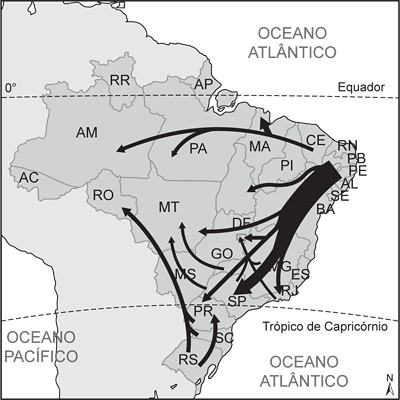
\includegraphics[width=\linewidth]{mapa_brasil_geografia.jpg}
\end{Figure}

		\begin{enumerate}
		\item  a marcha da industrializa\c{c}\~ao brasileira.
		\item o  fluxo de migra\c{c}\~oes no s\'eculo XX.
		\item o extrativismo mineral.
		\item as frentes pioneiras da agricultura brasileira.
		\item a nova expans\~ao industrial do s\'eculo XX.
		\end{enumerate}
%*e%
	\item Responda \`a quest\~ao com base na charge a seguir, referente \`a organiza\c{c}\~ao do mundo hoje.

\begin{Figure}
     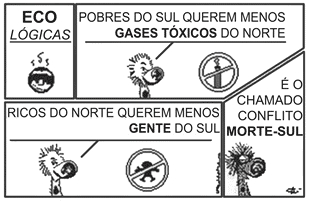
\includegraphics[width=\linewidth]{norte_sul_geografia.jpg}
\end{Figure}
		A charge:

		\begin{enumerate}
		\item representa uma divis\~ao esquem\'atica do mundo, representada pela linha do Equador, definida pela pobreza do Sul e riqueza do Norte.
		\item caracteriza uma realidade vivenciada no capitalismo industrial, onde a polui\c{c}\~ao foi o fator dominante devido \`a falta de tecnologia preventiva.
		\item mostra um conflito ideol\'ogico, e n\~ao econ\^omico, j\'a que representa a bipolariza\c{c}\~ao da Guerra Fria e a preocupa\c{c}\~ao com a ecologia.
		\item indica que, embora o Sul fique separado do Norte por uma linha imagin\'aria, h\'a uma n\'itida ruptura causada pelas diferen\c{c}as em administrar problemas ambientais.
		\item evidencia um antagonismo entre ricos e pobres, num conflito onde a popula\c{c}\~ao pobre dos pa\'ises do Sul \'e dominada pelo poder ideol\'ogico e econ\^omico do Norte.
		\end{enumerate}

%*d%
	\item Enquanto os piauienses est\~ao tomando o caf\'e da manh\~a, os italianos j\'a est\~ao almo\c{c}ando e os japoneses j\'a se preparam para o jantar. Isso ocorre porque foram estabelecidos diferentes fusos hor\'arios para os v\'arios pa\'ises do mundo, conforme a localiza\c{c}\~ao geogr\'afica de cada um, com base nas diferen\c{c}as de luminosidade decorrentes do movimento de rota\c{c}\~ao da Terra. Sobre essa quest\~ao, est\'a correto afirmar que:
		\begin{enumerate}
		\item todos os pa\'ises localizados ao longo de um mesmo paralelo t\^em o mesmo fuso hor\'ario.
		\item a Terra est\'a dividida em 24 faixas de meridianos, que equivalem a 15° cada uma, calculadas em rela\c{c}\~ao ao Equador, chamadas de fusos hor\'arios. 
		\item o estabelecimento da "hora legal" tem base nos fusos hor\'arios, considerando as faixas de 15° formadas pelos meridianos terrestres, enquanto a "hora local" tem base na posi\c{c}\~ao dos locais em rela\c{c}\~ao \`as suas latitudes.
		\item considerando que a Terra gira de oeste para leste, o Sol "nasce" primeiro nos pa\'ises de fusos hor\'arios a leste do meridiano zero. 
		\item cada fuso hor\'ario cont\'em paralelos de 15 graus, por isso ocorrem diferen\c{c}as de horas nos pa\'ises que se localizam no leste em rela\c{c}\~ao aos do oeste do globo terrestre.
		\end{enumerate}

%*d%
	\item  A can\c{c}\~ao e o gr\'afico retratam a desigualdade brasileira:
	\begin{quote}
		Os lucros s\~ao muito grandes, mas ningu\'em quer abrir m\~ao mesmo
		uma pequena parte j\'a seria solu\c{c}\~ao
		mas a usura dessa gente j\'a virou um aleij\~ao
		\^o\^o\^o\^o gente est\'upida, \^o\^o\^o\^o gente hip\'ocrita \footnote{GIL, Gilberto. Nos barracos da cidade, 1995.}
	\end{quote}

\begin{Figure}
     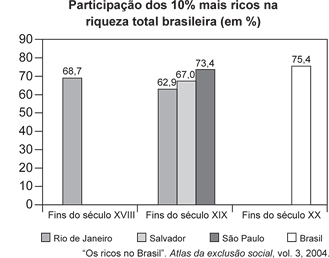
\includegraphics[width=\linewidth]{participacao_10_ricos_geografia.jpg}
\end{Figure}
	A alternativa que melhor expressa essa realidade \'e:
		\begin{enumerate}
		\item Os dados e a can\c{c}\~ao denunciam o Brasil contemporâneo como a pior distribui\c{c}\~ao de renda do globo, da\'i a refer\^encia \`a estupidez das pessoas.
		\item  A concentra\c{c}\~ao de renda no Brasil apresentou uma acentuada queda no final do s\'eculo XX.
		\item Salvador \'e a \'unica metr\'opole que n\~ao apresentou aumento da concentra\c{c}\~ao de renda, portanto, uma exce\c{c}\~ao no ``aleij\~ao" citado na can\c{c}\~ao.
		\item A ``usura" e a p\'essima distribui\c{c}\~ao de renda brasileira s\~ao uma heran\c{c}a colonial que pouco se alterou ao longo da hist\'oria brasileira.
		\item O gr\'afico indica uma expressiva melhora da situa\c{c}\~ao social do Brasil para o s\'eculo seguinte e, consequentemente, a desatualiza\c{c}\~ao futura da can\c{c}\~ao.
		\end{enumerate}

%*a%
	\item As atividades econ\^omicas na regi\~ao amaz\^onica, particularmente a pecu\'aria e o cultivo de soja, s\~ao respons\'aveis pela redu\c{c}\~ao de enormes \'areas de florestas. Que alternativa apresenta uma consequ\^encia irrevers\'ivel decorrente da falta da floresta original?
		\begin{enumerate}
		\item Redu\c{c}\~ao da biodiversidade, pois muitas esp\'ecies ainda desconhecidas desaparecer\~ao. 
		\item Redu\c{c}\~ao da vaz\~ao dos grandes rios da regi\~ao devida ao ac\'umulo de madeira no seu curso.
		\item Redu\c{c}\~ao da eros\~ao do solo gra\c{c}as ao aumento da produtividade agr\'icola da regi\~ao.
		\item Aumento do n\'umero de esp\'ecies na regi\~ao, pois a pecu\'aria e a soja atraem novos seres vivos para a \'area.
		\item Aumento da intensidade das chuvas que caem na regi\~ao, gerando grandes alagamentos.
		\end{enumerate}

%*d%
	\item ``A Funda\c{c}\~ao Seade (Funda\c{c}\~ao Sistema Estadual de An\'alise de Dados) divulgou nesta quinta-feira o resultado de pesquisa que aponta que o Estado de S\~ao Paulo tem a maior popula\c{c}\~ao negra do pa\'is. Outro estudo tamb\'em aponta que os homic\'idios atingem a popula\c{c}\~ao negra duas vezes mais que a popula\c{c}\~ao branca (...)a popula\c{c}\~ao negra entre 10 e 24 anos tem taxa de 120 mortes para 100 mil habitantes, entre a popula\c{c}\~ao branca a taxa \'e de 60,5 para 100 mil."\footnote{Fonte: folha on-line, Caderno Cotidiano, S\~ao Paulo 16/11/2005 (com adapta\c{c}ões)}

Mapa tem\'atico do munic\'ipio de S\~ao Paulo\footnote{Fonte: Adapt. Cepid-Fapesp / CEM – Cebrap, 2004.}

\begin{Figure}
     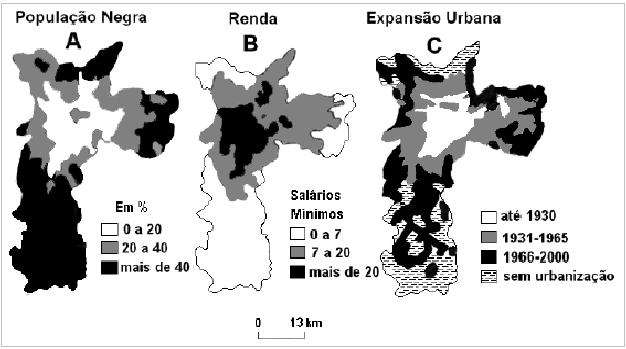
\includegraphics[width=\linewidth]{mapa_tematico_geografia.jpg}
\end{Figure}

Com base na leitura do texto e na an\'alise dos três mapas identifique a alternativa correta:

		\begin{enumerate}
		\item o texto e os mapas evidenciam que n\~ao existe  rela\c{c}\~ao entre a taxa de mortalidade e a renda da popula\c{c}\~ao negra.
		\item os mapas indicam que as maiores rendas (superior a 20 sal\'arios m\'inimos) apresentam-se na regi\~ao central da cidade de S\~ao Paulo coincidindo com a localiza\c{c}\~ao do maior percentual da popula\c{c}\~ao negra.
		\item a denominada regi\~ao perif\'erica, ou afastada do centro, abriga o alto \'indice de urbaniza\c{c}\~ao planejada e concretizada desde 1930.
		\item a leitura do texto e a observa\c{c}\~ao dos mapas permitem compreender que as maiores rendas concentram-se na regi\~ao central da cidade aonde encontramos os chamados bairros-chiques e planejados, como Jardim Paulista, Moema, Vila Mariana...
		\item existe apenas uma grande coincidência entre os mapas e o texto, pois n\~ao h\'a rela\c{c}\~ao social e hist\'orica  entre a urbaniza\c{c}\~ao planejada e a n\~ao planejada, a baixa renda da popula\c{c}\~ao e violência na cidade.
		\end{enumerate}

%*e%
	\item O lavrador de Ribeir\~ao Preto recebe em m\'edia R\$ 2,50 por tonelada de cana cortada. Nos anos 80, esse trabalhador cortava cinco toneladas de cana por dia. A mecaniza\c{c}\~ao da colheita o obrigou a ser mais produtivo. O corta-cana derruba agora oito toneladas por dia. O trabalhador deve cortar a cana rente ao ch\~ao, encurvado. Usa roupas mal-ajambradas, quentes, que lhe cobrem o corpo, para que n\~ao seja lanhado pelas folhas da planta. O excesso de trabalho causa a \emph{birola}: tontura, desmaio, c\~aibra, convuls\~ao. A fim de agüentar dores e cansa\c{c}o, esse trabalhador toma drogas e solu\c{c}ões de glicose, quando n\~ao farinha mesmo. Tem aumentado o n\'umero de mortes por exaust\~ao nos canaviais. \\
O setor da cana produz hoje uns 3,5\% do PIB. Exporta US\$ 8 bilhões. Gera toda a energia el\'etrica que consome e ainda vende excedentes. A ind\'ustria de S\~ao Paulo contrata cientistas e engenheiros para desenvolver m\'aquinas e equipamentos mais eficientes para as usinas de \'alcool. As pesquisas, privada e p\'ublica, na \'area agr\'icola (cana, laranja, eucalipto etc.) desenvolvem a bioqu\'imica e a gen\'etica no pa\'is. \footnote{Folha de S. Paulo, 11/3/2007 (com adapta\c{c}ões)}

\begin{Figure}
     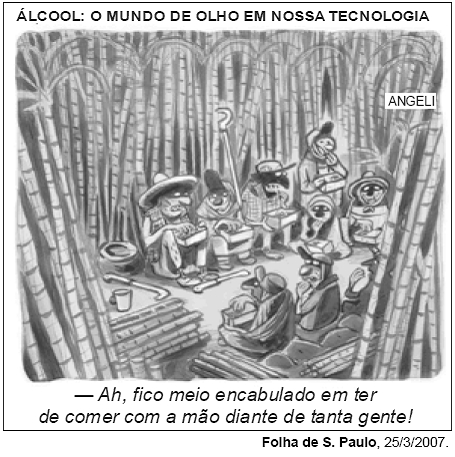
\includegraphics[width=\linewidth]{angeli_geografia.jpg}
\end{Figure}
Confrontando-se as informa\c{c}ões do texto com as da charge acima, conclui-se que

		\begin{enumerate}
		\item a charge contradiz o texto ao mostrar que o Brasil possui tecnologia avan\c{c}ada no setor agr\'icola.
		\item a charge e o texto abordam, a respeito da cana-de-a\c{c}\'ucar brasileira, duas realidades distintas e sem rela\c{c}\~ao entre si.
		\item o texto e a charge consideram a agricultura brasileira avan\c{c}ada, do ponto de vista tecnol\'ogico.
		\item a charge mostra o cotidiano do trabalhador, e o texto defende o fim da mecaniza\c{c}\~ao da produ\c{c}\~ao da cana-de-a\c{c}\'ucar no setor sucroalcooleiro.
		\item  o texto mostra disparidades na agricultura brasileira, na qual convivem alta tecnologia e condi\c{c}ões prec\'arias de trabalho, que a charge ironiza.
		\end{enumerate}

%*c%
	\item Sem que ningu\'em saiba como — e muito menos o por quê — uma catraca enferrujada foi colocada em cima de um pedestal no largo do Arouche (centro de S\~ao Paulo). \'E o ``monumento \`a catraca invis\'ivel", informa uma placa preta com moldura e letras douradas, colocada abaixo do objeto, onde se lê: ``Programa para a descatracaliza\c{c}\~ao da vida, Julho de 2004". \\
Um grupo art\'istico chamado Contra Fil\'e assumiu a responsabilidade pela coloca\c{c}\~ao da catraca. \footnote{Adaptado da Folha de S\~ao Paulo}

\begin{Figure}
     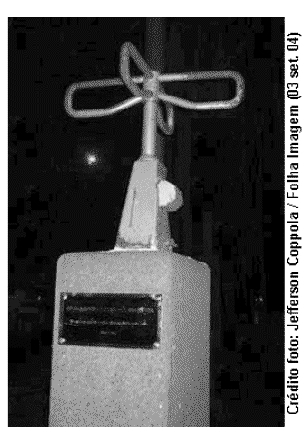
\includegraphics[width=\linewidth]{catraca_geografia.jpg}
\end{Figure}
	
	\begin{center} Arte e Vida \end{center}
	\begin{quote}
	A arte baseia-se na vida, por\'em n\~ao como mat\'eria mas como forma. Sendo a arte um produto directo do pensamento, \'e do pensamento que se serve como mat\'eria; a forma vai busc\'a-la \`a vida. A obra de arte \'e um pensamento tornado vida: um desejo realizado de si-mesmo. Como realizado tem que usar a forma da vida, que \'e essencialmente a realiza\c{c}\~ao; como realizado em si-mesmo tem que tirar de si a mat\'eria em que realiza.\footnote{ Fernando Pessoa, in 'Ricardo Reis - Prosa'}
	\end{quote}
	Mapa tem\'atico do munic\'ipio de S\~ao Paulo:

\begin{Figure}
     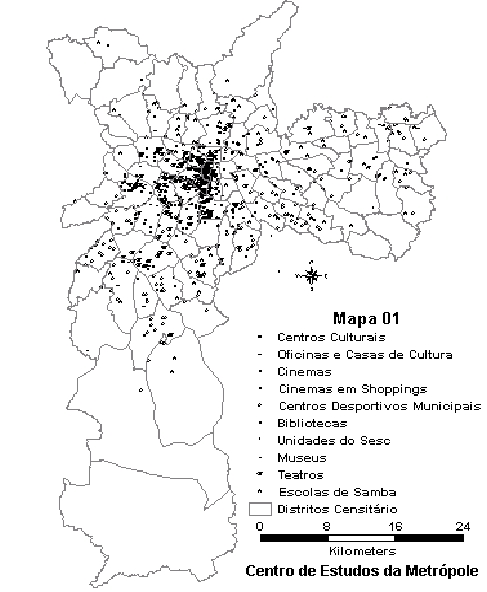
\includegraphics[width=\linewidth]{mapa_sao_paulo_geografia.jpg}
\end{Figure}
	
	Com base no texto, na prosa e  no mapa responda:

	\begin{enumerate}
		\item o grupo ``contra fil\'e" critica o pre\c{c}o da passagem de ônibus na cidade de S\~ao Paulo.
		\item existe um amplo oferecimento de diversas atividades culturais em todo munic\'ipio de S\~ao Paulo.
		\item a catraca, seja ela invis\'ivel ou real, representa o acesso restrito ou exclus\~ao social em diversos servi\c{c}os ou atividades da cidade, como transporte e cultura.
		\item segundo Fernando Pessoa a exposi\c{c}\~ao da catraca em cima de um pedestal n\~ao pode ser considerado uma obra de arte pois a catraca \'e um objeto presente no cotidiano e algo constante no dia a dia n\~ao deve receber tal aten\c{c}\~ao ou uma observa\c{c}\~ao mais cr\'itica.
		\item n.d.a.
	\end{enumerate}



	%%%%%%%%%%%%%%%%%%%%%%%%%%%%%%%%%%%%%%%%%%%%%%%%%%%%%%%%%%%%%%%%%%%%%%%%%%%%%%%%%%%%
	%%%%%%%%%%%  Biologia

%*c%
	\item Em certas \'epocas, na superf\'icie inferior das folhas das samambaias formam-se pontinhos escuros chamados \textbf{soros}. O surgimento dos soros indica que as samambaias est\~ao em \'epoca de reprodu\c{c}\~ao - em cada soro s\~ao produzidos in\'umeros \textbf{esporos}. \\
	Quando os esporos amadurecem, os soros se abrem. Ent\~ao os esporos caem no solo \'umido; cada esporo pode germinar e originar um protalo, como no esquema abaixo. \\
	O \textbf{ protalo} das samambaias cont\'em estruturas onde se formam \textbf{ anterozoides} e \textbf{ oosferas}. No interior do protalo existe \'agua em quantidade suficiente para que o anterozoide se desloque em meio l\'iquido e ``nade" em dire\c{c}\~ao \`a oosfera, fecundando-a. Surge ent\~ao o \textbf{ zigoto}, que se desenvolve e forma o embri\~ao. \\
	O \textbf{ embri\~ao}, por sua vez, se desenvolve e forma uma nova samambaia, isto \'e, um novo espor\'ofito. Quando adulta, as samambaias formam soros, iniciando novo ciclo de reprodu\c{c}\~ao. \footnote{http://www.sobiologia.com.br/conteudos/Reinos4/pteridofitas.php - adaptado}

\begin{Figure}
     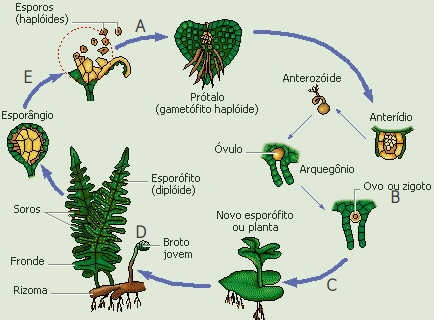
\includegraphics[width=\linewidth]{bio_ciclo.jpg}
\end{Figure}

	De acordo com o texto e esquema acima, assinale a alternativa correta:

		\begin{enumerate}
		\item No processo indicado pela letra A, ocorre meiose, uma vez que uma \'unica c\'elula haploide (chamada esporo) gera um indiv\'iduo multicelular tamb\'em haploide, o protalo
		\item O ovo ou zigoto, indicado pela letra B, \'e uma c\'elula haploide, uma vez que foi formado pela uni\~ao do \'ovulo e do anteroz\'oide
		\item No processo indicado pela letra C, ocorre mitose, uma vez que uma \'unica c\'elula diploide (chamada zigoto) gera um indiv\'iduo multicelular tamb\'em diploide, o espor \'ofito
		\item O broto jovem, indicado pela letra D, composto por c\'elulas diploides, continuar\'a crescendo, desenvolvendo o espor\'ofito, atrav\'es da meiose de suas c\'elulas 
		\item No processo indicado pela letra E, cada esporângio (diploide) gerar\'a, atrav\'es da meiose, dois esporos (haploides)
		\end{enumerate}

%*d%
	\item A figura seguinte representa um modelo de transmiss\~ao da informa\c{c}\~ao gen\'etica nos sistemas biol\'ogicos. No fim do processo, que inclui a replica\c{c}\~ao, a transcri\c{c}\~ao e a tradu\c{c}\~ao, h\'a tr\^es formas proteicas diferentes denominadas a, b e c.

\begin{Figure}
     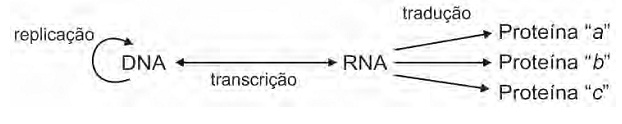
\includegraphics[width=\linewidth]{dna_rna_bio.jpg}
\end{Figure}

	Depreende-se do modelo que:

		\begin{enumerate}
		\item a \'unica mol\'ecula que participa da produ\c{c}\~ao de prote\'inas \'e o DNA
		\item o fluxo de informa\c{c}\~ao gen\'etica, nos sistemas biol\'ogicos, \'e unidirecional
		\item as fontes de informa\c{c}\~ao ativas durante o processo de transcri\c{c}\~ao s\~ao as prote\'inas
		\item \'e poss\'ivel obter diferentes variantes proteicas a partir de um mesmo produto de transcri\c{c}\~ao 
		\item a mol\'ecula de DNA possui forma circular e as demais mol\'eculas possuem forma de fita simples linearizadas
		\end{enumerate}

%*b%
	\item Alguns anf\'ibios e r\'epteis s\~ao adaptados \`a vida subterrânea. Nessa situa\c{c}\~ao, apresentam algumas caracter\'isticas corporais como, por exemplo, aus\^encia de patas, corpo anelado que facilita o deslocamento no subsolo e, em alguns casos, aus\^encia de olhos. \\
	Suponha que um bi\'ologo tentasse explicar a origem das adapta\c{c}\~oes mencionadas no texto utilizando conceitos da teoria evolutiva de Lamarck. Ao adotar esse ponto de vista, ele diria que:
		\begin{enumerate}
		\item as caracter\'isticas citadas no texto foram originadas por sele\c{c}\~ao natural
		\item a aus\^encia de olhos teria sido causada pela falta de uso dos mesmos, segundo a lei do uso e desuso.
		\item o corpo anelado \'e uma caracter\'istica fortemente adaptativa, mas seria transmitida apenas \`a primeira gera\c{c}\~ao de descendentes 
		\item as patas teriam sido perdidas pela falta de uso e, em seguida, essa caracter\'istica foi incorporada ao patrim\^onio gen\'etico e ent\~ao transmitida aos descendentes.
		\item as caracter\'isticas citadas no texto foram adquiridas por meio de muta\c{c}\~oes e depois, ao longo do tempo, foram selecionadas por serem mais adaptadas ao ambiente em que os organismos se encontram
		\end{enumerate}
%*a%
	\item Os espermatozoides s\~ao muito desiguais. Na escola, aprendemos que todos nadam alucinados atr\'as do \'ovulo, mas parece que n\~ao \'e t\~ao simples: os espermatozoides trabalham em conjunto, cada qual com uma fun\c{c}\~ao definida, como se fossem um ex\'ercito de guerreiros disciplinados. \\
	De acordo com essa hip\'otese, existiriam tr\^es grandes grupos de espermatozoides: \\
	1) \emph{pelot\~ao de elite}: seleto grupo de nadadores imbat\'iveis na velocidade. Armazenam a energia necess\'aria para o percurso em corp\'usculos situados na cabe\c{c}a comprida e t\^em cauda longa e \'agil. S\~ao poucos: cerca de 1\% dos milh\~oes ejaculados; \\
	2) \emph{bloqueadores}: t\^em cabe\c{c}a grande e cauda pequena. Nadam devagar; n\~ao v\~ao atr\'as do \'ovulo; s\~ao “camicases”: ao penetrar os canais do muco uterino, agarram-se \`as paredes para obstruir a passagem dos que v\^em atr\'as. A fun\c{c}\~ao bloqueadora ocupa cerca de 50\% dos espermatozoides; \\
	3) \emph{matadores}: carregam enzimas t\'oxicas na cabe\c{c}a e possuem antenas capazes de detectar e reconhecer espermatozoides estranhos. Quando os encontram, despejam neles suas enzimas mortais. Constituem praticamente a outra metade da popula\c{c}\~ao do esperma. \footnote{http://drauziovarella.com.br/sexualidade/a-estrategia-dos-espermatozoides/}\\
	De acordo com o texto acima, assinale a alternativa correta:
		\begin{enumerate}
		\item os espermatozoides pertencentes ao grupo 1 devem possuir um alto n\'umero de mitoc\^ondrias, j\'a que estas organelas s\~ao respons\'aveis pela s\'intese de ATP, mol\'ecula que armazena energia
		\item os espermatozoides pertencentes ao grupo 2 devem possuir um ret\'iculo endoplasm\'atico rugoso muito desenvolvido, uma vez que \'e nessa organela que se realiza a s\'intese de lip\'ideos, que ir\~ao formar a membrana celular
		\item os espermatozoides pertencentes ao grupo 3 devem possuir um ret\'iculo endoplasm\'atico liso muito desenvolvido, uma vez que \'e nessa organela que se realiza a s\'intese das enzimas t\'oxicas, um tipo de prote\'ina
		\item as enzimas t\'oxicas carregadas pelos espermatozoides pertencentes ao grupo 3, citadas no texto, ficam armazenadas dentro do lisossomo e tem a fun\c{c}\~ao de realizar a digest\~ao intracelular
		\item o DNA de um espermatozoides de um dos grupos deve ser necessariamente id\^entico ao de qualquer outro espermatozoide do mesmo grupo
		\end{enumerate}


	\item No esquema abaixo, as setas numeradas de I a IV indicam transfer\^encias de mol\'eculas ou energia entre seres vivos e entre eles e o ambiente.

\begin{Figure}
     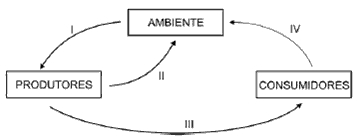
\includegraphics[width=\linewidth]{transferencia_bio.jpg}
\end{Figure}

	Assinale a alternativa do quadro abaixo que mostra, corretamente, as passagens em que h\'a transfer\^encia de g\'as carb\^onico, de mol\'eculas orgânicas ou de energia.

\begin{Figure}  % tabela com as alternativas
	\begin{tabular}{|c|c|c|c|} % aqui temos 4 colunas centralizadas
	\hline
	& \multicolumn{2}{c}{Transfer\^encia de energia e mol\'eculas} & \tabularnewline
	
	\hline
	  & G\'as carb\^onico & Mol\'eculas orgânicas & Energia \tabularnewline

	\hline
		a) & I e II & I e IV & I e III \tabularnewline
	\hline
		b) & I e IV & II & I, III e IV \tabularnewline
	\hline
		c) & I, II e IV & III & I, II, III e IV \tabularnewline
	\hline
		d) & I, II e III & III e IV & I, II, III e IV \tabularnewline
	\hline
		e) & II, III e IV & II e III & I e II \tabularnewline
	\hline
	\end{tabular}
\end{Figure}


	\item De 15\% a 20\% da \'area de um canavial precisa ser renovada anualmente. Entre o per\'iodo de corte e o de planta\c{c}\~ao de novas canas, os produtores est\~ao optando por plantar leguminosas, pois elas fixam nitrog\^enio no solo, um adubo natural para a cana. Essa op\c{c}\~ao de rota\c{c}\~ao \'e agronomicamente favor\'avel, de forma que munic\'ipios canavieiros s\~ao hoje grandes produtores de soja, amendoim e feij\~ao. \footnote{As encruzilhadas da fome. Planeta. S\~ao Paulo, ano 36, nº.430, jul.2008 (adaptado)} \\
	A rota\c{c}\~ao de culturas citada no texto pode beneficiar economicamente os produtores de cana porque:

		\begin{enumerate}
		\item a decomposi\c{c}\~ao da cobertura morta dessas culturas resulta em economia na aquisi\c{c}\~ao de adubos industrializados.
		\item o plantio de cana-de-a\c{c}\'ucar propicia um solo mais adequado para o cultivo posterior de soja, do amendoim e do feij\~ao.
		\item as leguminosas absorvem do solo elementos qu\'imicos diferentes dos absorvidos pela cana, restabelecendo o equil\'ibrio do solo. 
		\item a queima dos restos vegetais do cultivo da cana-de-a\c{c}\'ucar transforma-se em cinzas, sendo reincorporadas ao solo, o que gera economia na aquisi\c{c}\~ao de adubo. 
		\item a soja, o amendoim e o feij\~ao, al\'em de possibilitarem a incorpora\c{c}\~ao ao solo de determinadas mol\'eculas dispon\'iveis na atmosfera, s\~ao gr\~aos comercializados no mercado produtivo.
		\end{enumerate}

\pagebreak

	\item A figura a seguir ilustra as principais fontes de emiss\~oes mundiais de g\'as carb\^onico, relacionando as a nossas compras dom\'esticas (familiares).

\begin{Figure}
     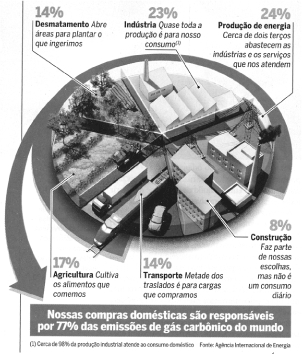
\includegraphics[width=\linewidth]{poluicao_consumo_bio.jpg}
\end{Figure}

Com base nas informa\c{c}\~oes da figura, \'e observado que as emiss\~oes de g\'as carb\^onico est\~ao diretamente ligadas \`as compras dom\'esticas. Deste modo, deduz-se das rela\c{c}\~oes de produ\c{c}\~ao e consumo apresentadas que:

		\begin{enumerate}
		\item  crescimento econ\^omico e prote\c{c}\~ao ambiental s\~ao pol\'iticas p\'ublicas incompat\'iveis.
		\item a redu\c{c}\~ao da atividade industrial teria pouco impacto nas emiss\~oes globais de g\'as carb\^onico.
		\item os fluxos de carbono na biosfera n\~ao s\~ao afetados pela atividade humana, pois s\~ao processos c\'iclicos.
		\item a produ\c{c}\~ao de alimentos, em seu conjunto, \'e diretamente respons\'avel por 17\% das emiss\~oes de g\'as carb\^onico.
		\item haveria decr\'escimo das emiss\~oes de g\'as carb\^onico se o consumo ocorresse em \'areas mais pr\'oximas da produ\c{c}\~ao. 
		\end{enumerate}



\end{enumerate}

\end{multicols}

% \vspace{2pc} \hrule \vspace{1pc} \hrule

\end{document}
